\documentclass[article,shortnames]{jss}\usepackage[]{graphicx}\usepackage[]{color}
% maxwidth is the original width if it is less than linewidth
% otherwise use linewidth (to make sure the graphics do not exceed the margin)
\makeatletter
\def\maxwidth{ %
  \ifdim\Gin@nat@width>\linewidth
    \linewidth
  \else
    \Gin@nat@width
  \fi
}
\makeatother

\definecolor{fgcolor}{rgb}{0.345, 0.345, 0.345}
\newcommand{\hlnum}[1]{\textcolor[rgb]{0.686,0.059,0.569}{#1}}%
\newcommand{\hlstr}[1]{\textcolor[rgb]{0.192,0.494,0.8}{#1}}%
\newcommand{\hlcom}[1]{\textcolor[rgb]{0.678,0.584,0.686}{\textit{#1}}}%
\newcommand{\hlopt}[1]{\textcolor[rgb]{0,0,0}{#1}}%
\newcommand{\hlstd}[1]{\textcolor[rgb]{0.345,0.345,0.345}{#1}}%
\newcommand{\hlkwa}[1]{\textcolor[rgb]{0.161,0.373,0.58}{\textbf{#1}}}%
\newcommand{\hlkwb}[1]{\textcolor[rgb]{0.69,0.353,0.396}{#1}}%
\newcommand{\hlkwc}[1]{\textcolor[rgb]{0.333,0.667,0.333}{#1}}%
\newcommand{\hlkwd}[1]{\textcolor[rgb]{0.737,0.353,0.396}{\textbf{#1}}}%
\let\hlipl\hlkwb

\usepackage{framed}
\makeatletter
\newenvironment{kframe}{%
 \def\at@end@of@kframe{}%
 \ifinner\ifhmode%
  \def\at@end@of@kframe{\end{minipage}}%
  \begin{minipage}{\columnwidth}%
 \fi\fi%
 \def\FrameCommand##1{\hskip\@totalleftmargin \hskip-\fboxsep
 \colorbox{shadecolor}{##1}\hskip-\fboxsep
     % There is no \\@totalrightmargin, so:
     \hskip-\linewidth \hskip-\@totalleftmargin \hskip\columnwidth}%
 \MakeFramed {\advance\hsize-\width
   \@totalleftmargin\z@ \linewidth\hsize
   \@setminipage}}%
 {\par\unskip\endMakeFramed%
 \at@end@of@kframe}
\makeatother

\definecolor{shadecolor}{rgb}{.97, .97, .97}
\definecolor{messagecolor}{rgb}{0, 0, 0}
\definecolor{warningcolor}{rgb}{1, 0, 1}
\definecolor{errorcolor}{rgb}{1, 0, 0}
\newenvironment{knitrout}{}{} % an empty environment to be redefined in TeX

\usepackage{alltt}

%% -- LaTeX packages and custom commands ---------------------------------------

%% recommended packages
\usepackage{thumbpdf,lmodern}
\usepackage{amsmath, amsfonts}
\usepackage{bbm}% to get \mathbbmm{1}

%% another package (only for this demo article)
\usepackage{booktabs}
\usepackage{adjustbox}
\usepackage{tabularx}
\usepackage{rotating}

%% packages for the table
\usepackage{booktabs}
\usepackage{array}
\usepackage{pdflscape}
\usepackage{float}
\usepackage{longtable}
\usepackage{multirow}

\usepackage{xcolor}
\usepackage{colortbl}


%% packages for landscape
%% there are probably duplicates
\usepackage{array}
\usepackage{pdflscape}
\usepackage{amsfonts}
\usepackage{amsmath}
\usepackage{xcolor}
\usepackage{colortbl}
\usepackage{float}
\usepackage{longtable}

%% new custom commands
\newcommand{\class}[1]{`\code{#1}'}
\newcommand{\fct}[1]{\code{#1()}}

%% For Sweave-based articles about R packages:
%% need no \usepackage{Sweave}






%% -- Article metainformation (author, title, ...) -----------------------------

%% - \author{} with primary affiliation
%% - \Plainauthor{} without affiliations
%% - Separate authors by \And or \AND (in \author) or by comma (in \Plainauthor).
%% - \AND starts a new line, \And does not.
\author{Nikos I. Bosse\\London School of Hygiene and Tropical Medicine
   \And Second Author\\Plus Affiliation}
\Plainauthor{Nikos I. Bosse, Second Author}

%% - \title{} in title case
%% - \Plaintitle{} without LaTeX markup (if any)
%% - \Shorttitle{} with LaTeX markup (if any), used as running title
\title{Evaluating Covid-19 Short-Term Forecasts using \pkg{scoringutils} in \proglang{R}}
\Plaintitle{Evaluating Covid-19 Short-Term Forecasts using scoringutils in R}
\Shorttitle{Evaluating Forecasts with \pkg{scoringutils} in \proglang{R}}

%% - \Abstract{} almost as usual
\Abstract{
  Forecasts play an important role in a variety of fields. Their role in informing public policy has attracted increased attention from the general public with the emergence of the Covid-19 pandemic. Much theoretical work has been done on the development of proper scoring rules and other scoring metrics that can help evaluate these forecasts. Making these theoretical insights available to end users, however, has been less of a focus. In this paper we introduce \pkg{scoringutils}, an \proglang{R} package that facilitates automated forecast evaluation. It gives the user access to a wide range of scoring metrics for various types of forecasts as well as a variety of ways to visualise the evaluation. We give an overview of the evaluation process and the metrics implemented in \pkg{scoringutils} and show an example evaluation of forecasts for COVID-19 cases and deaths submitted to the European Forecast Hub between May und September 2021. 
}

%% - \Keywords{} with LaTeX markup, at least one required
%% - \Plainkeywords{} without LaTeX markup (if necessary)
%% - Should be comma-separated and in sentence case.
\Keywords{JSS, style guide, comma-separated, not capitalized, \proglang{R}}
\Plainkeywords{JSS, style guide, comma-separated, not capitalized, R}

%% - \Address{} of at least one author
%% - May contain multiple affiliations for each author
%%   (in extra lines, separated by \emph{and}\\).
%% - May contain multiple authors for the same affiliation
%%   (in the same first line, separated by comma).
\Address{
  Nikos Bosse\\
  Centre for Mathematical Modelling of Infectious Diseases\\
  London School of Hygiene and Tropical Medicine\\
  Keppel Street \\ 
  London WC1E 7HT \\
  E-mail: \email{nikos.bosse@lshtm.ac.uk}\\
  % URL: \url{https://eeecon.uibk.ac.at/~zeileis/}
}
\IfFileExists{upquote.sty}{\usepackage{upquote}}{}
\begin{document}





%% -- Introduction -------------------------------------------------------------

%% - In principle "as usual".
%% - But should typically have some discussion of both _software_ and _methods_.
%% - Use \proglang{}, \pkg{}, and \code{} markup throughout the manuscript.
%% - If such markup is in (sub)section titles, a plain text version has to be
%%   added as well.
%% - All software mentioned should be properly \cite-d.
%% - All abbreviations should be introduced.
%% - Unless the expansions of abbreviations are proper names (like "Journal
%%   of Statistical Software" above) they should be in sentence case (like
%%   "generalized linear models" below).

\section[Introduction]{Introduction}
Good forecasts are of great interest to decision makers in various fields like finance \citep{timmermannForecastingMethodsFinance2018} [CITATION], weather predictions [CITATION] or infectious disease modeling \citep{funkShorttermForecastsInform2020} [CITATIONS]. An integral part of assessing and improving their usefulness is forecast evaluation. For decades, researchers have developed and refined an arsenal of techniques not only to forecast, but also to evaluate these forecasts (see e.g. \cite{bracherEvaluatingEpidemicForecasts2021}, \cite{funkAssessingPerformanceRealtime2019}, \cite{gneitingProbabilisticForecastsCalibration2007}, and \cite{gneitingStrictlyProperScoring2007}). Yet even with this rich body of research available, implementing a complete forecast evaluation in \proglang{R} is not trivial. 

Some packages exist that bundle different scoring metrics together, but none offer the user a standalone solution to forecast evaluation. The \pkg{scoringRules} package \citep{scoringRules} offers a very extensive collection of proper scoring rules. Its exclusive focus on proper scoring rules and the fact that all functions are implemented using vectors and matrices instead of data.frames, however, make it more suitable for experienced users or as a building block in larger application. It also lacks features like pairwise comparisons between forecast models and plotting functionality that are invaluable in the evaluation process. Other packages like \pkg{Metrics} [https://cran.r-project.org/web/packages/Metrics/Metrics.pdf] \pkg{MLmetrics} [https://cran.r-project.org/web/packages/MLmetrics/MLmetrics.pdf] are geared towards machine learning problems and don't implement the set of metrics and scoring rules desired for forecast evaluation. The \pkg{scoringutils} package aims to bring forth a standardised and tested toolkit. It offers convenient automated forecast evaluation in a data.table format, but also provides experienced users with a set of reliable lower-level scoring metrics they can build upon in other applications. In addition it implements a wide range of flexible plots that are able to cover most day-to-day use cases. 

This paper provides an overview of the fundamental ideas behind forecast evaluation, gives a detailed explanation of the evaluation metrics in \pkg{scoringutils} and discusses what to think about when applying them in practice. It then presents a case study based on the evaluation of Covid-19 related short-term forecasts in the UK \citep{funkShorttermForecastsInform2020}. 
\subsection{Forecast types and forecast formats}

In its most general sense, a forecast is the forecaster’s stated belief about the future \citep{gneitingStrictlyProperScoring2007} that can come in many different forms. Quantitative forecasts are either point forecasts or probabilistic in nature and can make statements about continuous, discrete or binary outcome variables. Point forecasts only give one single number for the most likely outcome, but do not quantify the forecaster's uncertainty. This limits their usefulness, as a very certain forecast may, for example, warrant a very different course of actions than does a very uncertain one. Probabilistic forecasts, in contrast, by definition provide a full predictive distribution. This makes them much more useful in any applied setting, as we learn about the forecaster's uncertainty and their belief about all aspects of the underlying data-generating distribution (including e.g. skewness or the width of its tails). Probabilistic forecasts are therefore the focus of this paper as well as the \pkg{scoringutils} package. 

The predictive distribution of a probabilistic forecast can be represented in different ways with implications for the appropriate evaluation approach. For most forecasting problems, predictive distributions are not readily available in a closed form (and the \pkg{scoringutils} package therefore does not support scoring them directly). Instead, predictive distributions are often represented by a set of quantiles or predictive samples. Predictive samples require a lot of storage space and also come with a loss of precision that is especially pronounced in the tails of the predictive distribution, where quite a lot of samples are needed to accurately characterise the distribution. For that reason, often quantiles or central prediction intervals are reported instead [citation FORECAST HUBS]. For binary or multinomial prediction targets, common in many classification problems, a probabilistic forecasts is represented by the probability that an outcome will come true. Table \ref{tab:forecast-types} summarises the different forecast types and formats. While specific metrics may differ depending on the forecast type or format, the general forecasting paradigm \cite{gneitingProbabilisticForecastsCalibration2007} that guides the evaluation process is the same.

\begin{table}[h!]
\centering

\begin{longtable}[t]{>{\raggedright\arraybackslash}p{3.5cm}>{\raggedright\arraybackslash}p{2.5cm}>{\raggedright\arraybackslash}p{4.5cm}}
\toprule
\textbf{Forecast type} & \textbf{Target type} & \textbf{Representation of the predictive distribution}\\
\midrule
Point forecast & continuous \newline  discrete \newline  binary & one single number for the predicted outcome\\
\cmidrule{1-3}\pagebreak[0]
 & continuous \newline  discrete & predictive samples \newline   quantiles \newline   closed analytical form\\
\cmidrule{2-3}\nopagebreak
\multirow{-2}{3.5cm}{\raggedright\arraybackslash Probabilistic forecast} & binary & binary probabilities\\
\bottomrule
\end{longtable}


\caption{\label{tab:forecast-types} Forecasts can be distinguished by whether they are probabilistic in nature, or a point forecast only. Depending on the type of the target (discrete, continuous or binary) different representation of the predictive distribution are possible.} 
\end{table}


\subsection{The forecasting paradigm}

Any forecaster should aim to minimise the difference between the (cumulative) predictive distribution $F$ and the unknown true data-generating distribution $G$ \citep{gneitingProbabilisticForecastsCalibration2007}. For an ideal forecast, we therefore have 
%
$$ F = G, $$
%
where $F$ and $G$ are both cumulative distribution functions. As we don't know the true data-generating distribution, we cannot assess the difference between the two distributions directly. \cite{gneitingProbabilisticForecastsCalibration2007} instead suggest to focus on two central aspects of the predictive distribution, calibration and sharpness (illustrated in Figure \ref{fig:forecast-paradigm}. Calibration refers to the statistical consistency (i.e. absence of systematic deviations) between the predictive distribution and the observations. Sharpness is a feature of the forecast only and describes how concentrated the predictive distribution is, i.e. how precise the forecasts are. The general forecasting paradigm states that we should maximise sharpness of the predictive distribution subject to calibration. A model that made very precise forecasts would at best be useless if the forecasts were wrong most of the time. On the other hand, a model may be well calibrated, but not sharp enough to be useful. Take a weather forecast that would assign 30 percent rain probability for every single day. It may be (marginally) calibrated when looking at the average rainfall over the course of a year, but it doesn't give much guidance on a day to day basis. \cite{gneitingProbabilisticForecastsCalibration2007} discuss different forms of calibration in more detail. 

\begin{figure}[h]
\centering
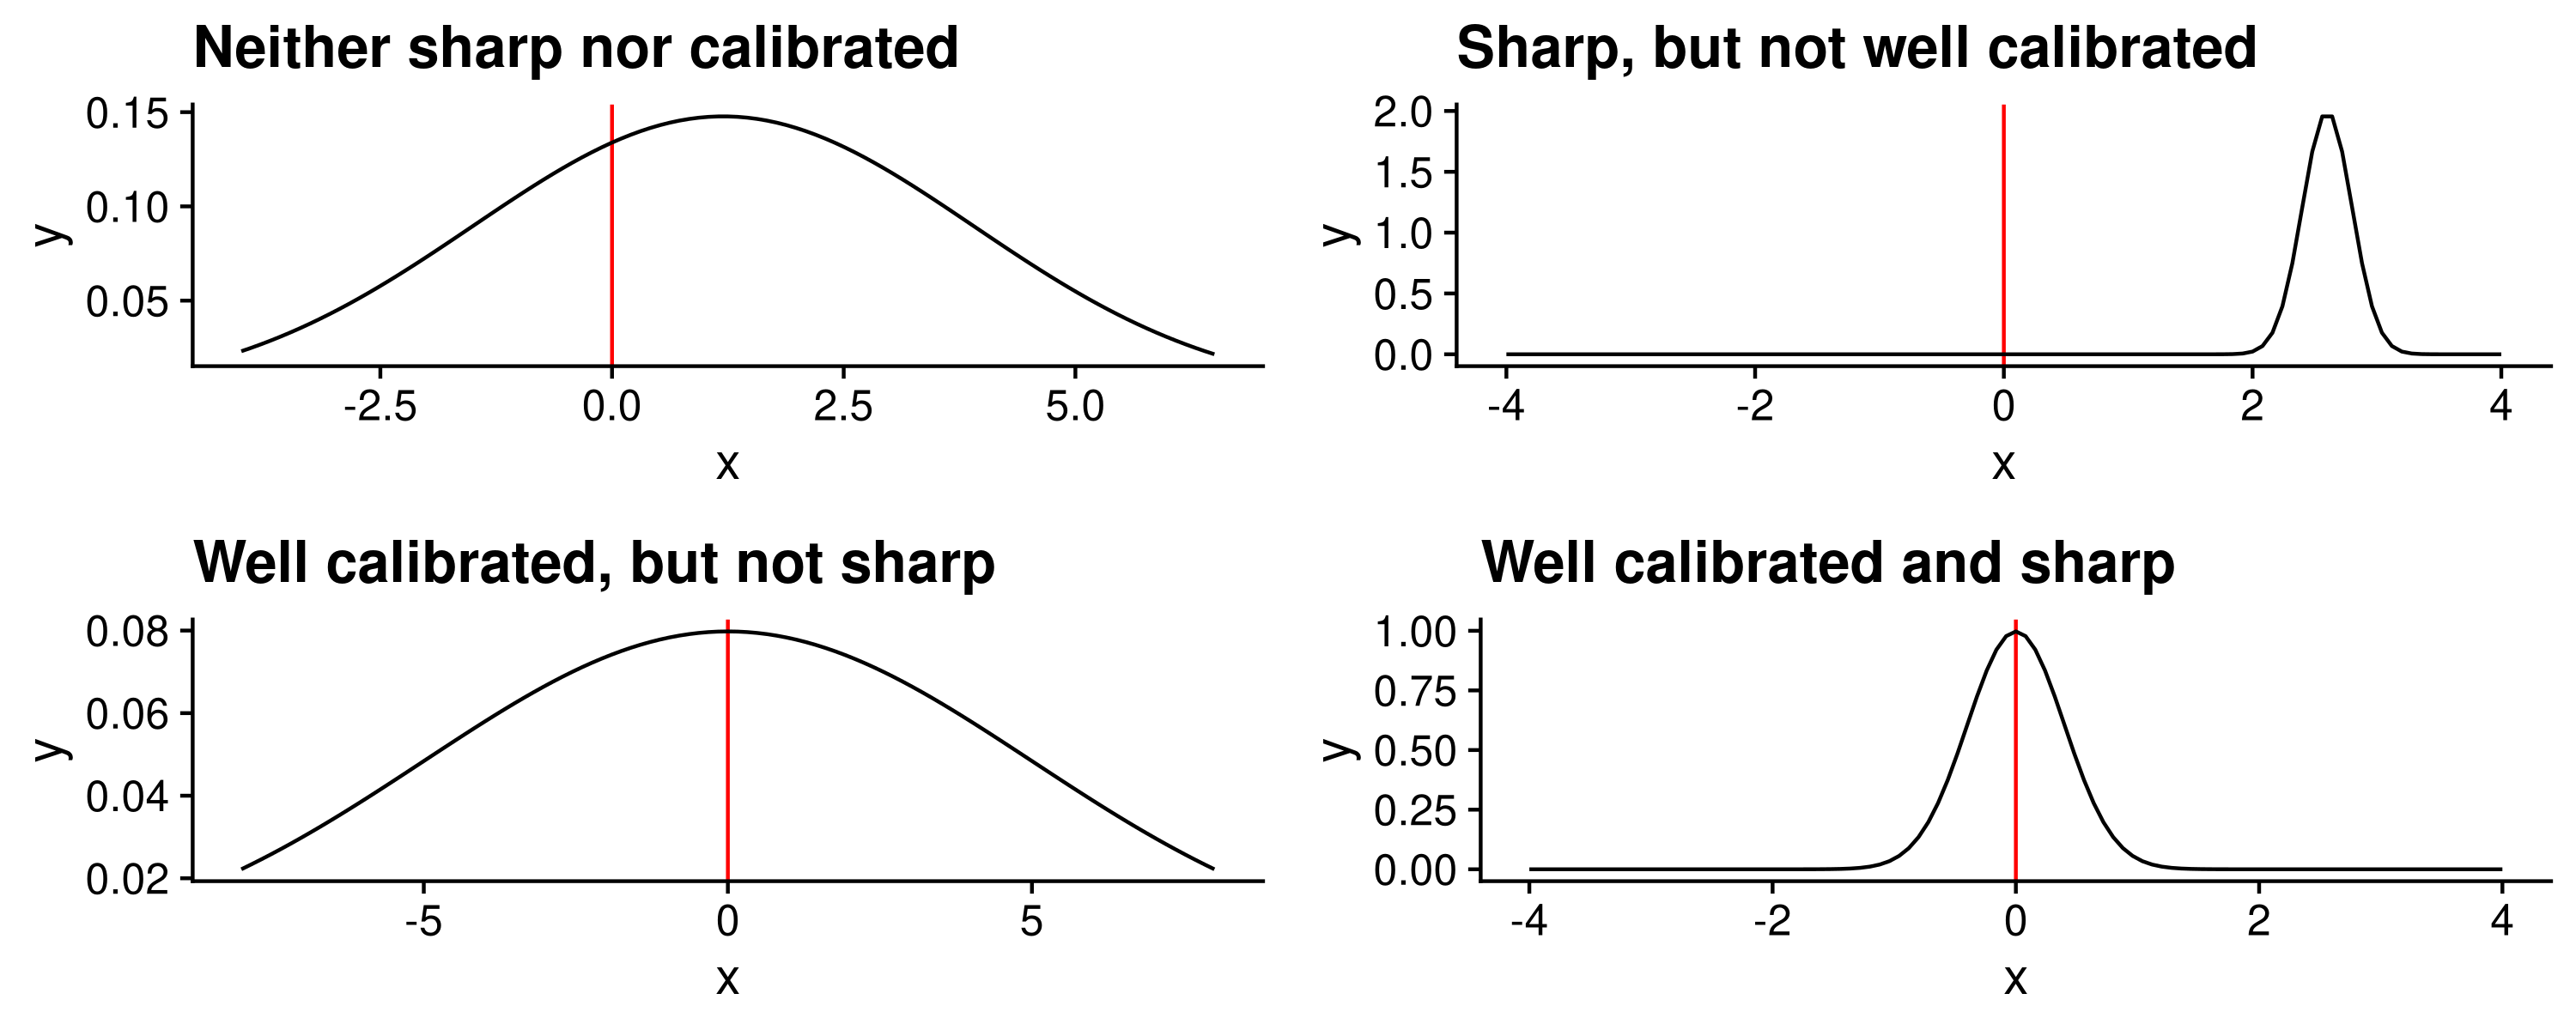
\includegraphics{plots/forecast-paradigm.png}
\caption{\label{fig:forecast-paradigm} Schematic illustration of calibration and sharpness. True value are represented in red, the predictive distribution is shown in black}
\end{figure}


% ==============================================================================
\section[metrics]{Scoring metrics implemented in \pkg{scoringutils}}

Some of the metrics in \pkg{scoringuitls} focus only on sharpness or on calibration. Others, called proper scoring rules, combine both aspects into a single number. The former can be helpful to learn about specific model aspects and improve them, the latter are especially useful to assess and rank predictive performance of a forecaster. The following gives an introduction to how these metrics can be used to evaluate forecasts. Table \ref{tab:table-summary-scores} shows an overview of the metrics implemented in \pkg{scoringutils}. Table \ref{tab:score-table} in the Appendix gives a mathematical definition and thorough explanation of all the metrics. Figure \ref{fig:calibration-plots} gives an applied example of different scoring metrics and visualisations for simple toy data. 

% \begin{table}[h!]
% \centering

\newpage
\begin{table}[h!]
\centering
\begingroup\fontsize{8}{10}\selectfont

\begin{longtable}[t]{>{\raggedright\arraybackslash}p{1.8 cm}>{\centering\arraybackslash}p{1.2cm}>{\centering\arraybackslash}p{1.2cm}>{\centering\arraybackslash}p{1.0cm}>{\centering\arraybackslash}p{1.0cm}>{\centering\arraybackslash}p{1.3cm}>{\centering\arraybackslash}p{1.1cm}>{\raggedright\arraybackslash}p{3.4cm}}
\toprule
Metric & Discrete & Continuous & Binary & Closed-form & Samples (approx.) & Quantiles & Properties\\
\midrule
\cellcolor{gray!6}{(Continuous) ranked probability score (CRPS)} & \cellcolor{gray!6}{$\checkmark$} & \cellcolor{gray!6}{$\checkmark$} & \cellcolor{gray!6}{} & \cellcolor{gray!6}{$\checkmark$} & \cellcolor{gray!6}{$\checkmark$} & \cellcolor{gray!6}{} & \cellcolor{gray!6}{proper scoring rule, global, stable handling of outliers}\\
\addlinespace
Log score (logS) &  & $\checkmark$ &  & $\checkmark$ & $\checkmark$ &  & proper scoring rule, log of predictive density evaluated at observed value, local, unstable for outliers\\
\addlinespace
\cellcolor{gray!6}{(Weighted) interval score (WIS)} & \cellcolor{gray!6}{$\checkmark$} & \cellcolor{gray!6}{$\checkmark$} & \cellcolor{gray!6}{} & \cellcolor{gray!6}{} & \cellcolor{gray!6}{THINK} & \cellcolor{gray!6}{$\checkmark$} & \cellcolor{gray!6}{proper scoring rule, global, stable handling of outliers, converges to crps for an increasing numbre of equally spaced intervals}\\
\addlinespace
Dawid-Sebastiani score (DSS) & $\checkmark$ & $\checkmark$ &  & $\checkmark$ & $\checkmark$ &  & proper scoring rule, somewhat global, somewhat stable handling of outliers\\
\addlinespace
\cellcolor{gray!6}{Brier score (BS)} & \cellcolor{gray!6}{} & \cellcolor{gray!6}{} & \cellcolor{gray!6}{$\checkmark$} & \cellcolor{gray!6}{} & \cellcolor{gray!6}{$\checkmark$} & \cellcolor{gray!6}{} & \cellcolor{gray!6}{proper scoring rule}\\
\addlinespace
Interval coverage & $\checkmark$ & $\checkmark$ &  &  & THINK & $\checkmark$ & measure for calibration\\
\addlinespace
\cellcolor{gray!6}{Quantile coverage} & \cellcolor{gray!6}{$\checkmark$} & \cellcolor{gray!6}{$\checkmark$} & \cellcolor{gray!6}{} & \cellcolor{gray!6}{} & \cellcolor{gray!6}{THINK} & \cellcolor{gray!6}{$\checkmark$} & \cellcolor{gray!6}{measure for calibration}\\
\addlinespace
Probability integral transform (PIT) & $\checkmark$ & $\checkmark$ &  & $\checkmark$ & $\checkmark$ & $\checkmark$ & assesses calibration\\
\addlinespace
\cellcolor{gray!6}{Sharpness} & \cellcolor{gray!6}{$\checkmark$} & \cellcolor{gray!6}{$\checkmark$} & \cellcolor{gray!6}{} & \cellcolor{gray!6}{$\checkmark$} & \cellcolor{gray!6}{$\checkmark$} & \cellcolor{gray!6}{$\checkmark$} & \cellcolor{gray!6}{measures forecast dispersions}\\
\addlinespace
Bias & $\checkmark$ & $\checkmark$ & $\checkmark$??? & $\checkmark$ & $\checkmark$ & $\checkmark$ & captures tendency to over-or underpredict (aspect of calibration)\\
\addlinespace
\cellcolor{gray!6}{Mean score ratio} & \cellcolor{gray!6}{$\sim$} & \cellcolor{gray!6}{$\sim$} & \cellcolor{gray!6}{$\sim$} & \cellcolor{gray!6}{$\sim$} & \cellcolor{gray!6}{$\sim$} & \cellcolor{gray!6}{$\sim$} & \cellcolor{gray!6}{compares performance of two models. Properties depend on the metric chosen for the comparison.}\\
\addlinespace
Relative skill & $\sim$ & $\sim$ & $\sim$ & $\sim$ & $\sim$ & $\sim$ & Ranks models based on pairwise comparisons. Properties depend on the metric chosen for the comparison.\\
\bottomrule
\end{longtable}
\endgroup{}


\caption{\label{tab:table-summary-scores2} Summary table of scores available in scoringutils}
\end{table}

\newpage







\begin{figure}[h]
\centering
\begin{knitrout}
\definecolor{shadecolor}{rgb}{0.969, 0.969, 0.969}\color{fgcolor}
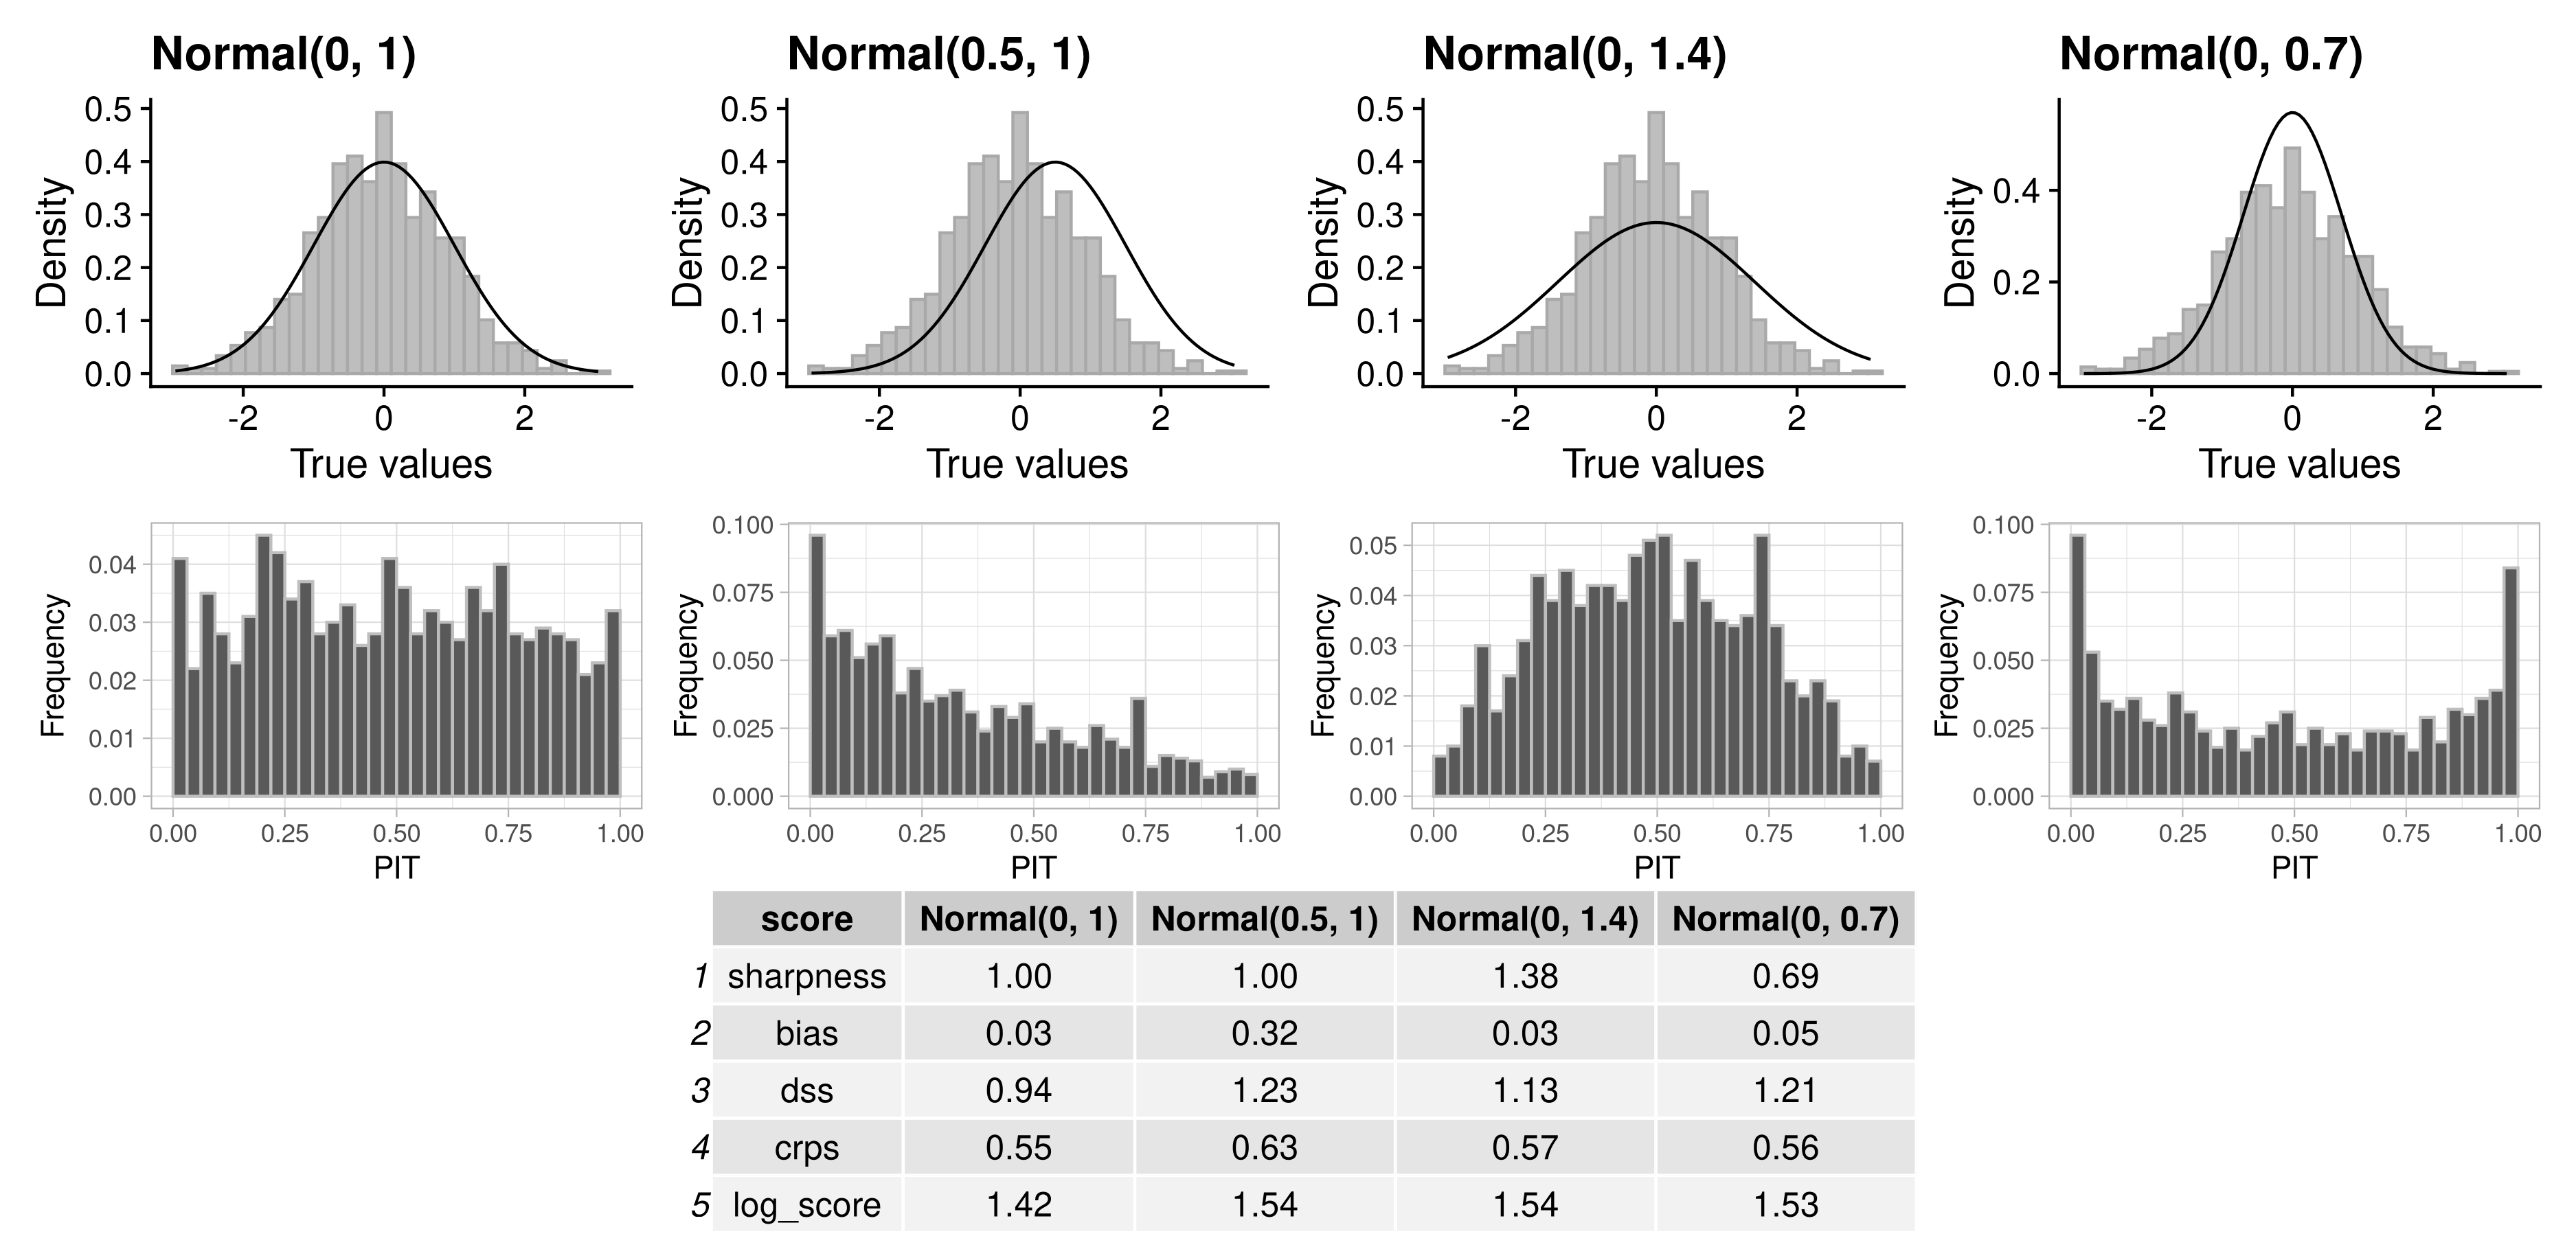
\includegraphics[width=\maxwidth]{/mnt/data/GoogleDrive/Uni/PhD/scoringutils-paper/plots/calibration-diagnostic-examples} 
\end{knitrout}

\caption{\label{fig:calibration-plots} Calibration plots for different forecast distributions. I plan to add interval and quantile coverage plots, but these still have to be made.}
\end{figure}

\subsection{Evaluating calibration and sharpness independently}

Evaluating calibration and sharpness independently is helpful for model diagnostics. To that end \pkg{scoringutils} makes numerous metrics available that aim to capture different aspects of sharpness and calibration. 

\subsubsection{Assessing calibration} 

Calibration means consistency between forecasts and observed values, but there are various ways in which a forecast can systematically deviate from the observations (see \cite{gneitingProbabilisticForecastsCalibration2007} for a discussion of different forms of calibration MAYBE IT WOULD BE A GOOD IDEA TO INCLUDE THESE DIFFERENT FORMS OF CALIBRATION HERE).
\pkg{scoringutils} allows the user to examine three different sub-aspects of calibration: bias, empirical coverage, and the probability integral transform (PIT). 

% Bias
Bias, i.e. systematic over- or underprediction, is a very common form of miscalibration which therefore deserves separate attention. The bias metric (with slightly different versions for the various forecast types and formats) captures a general tendency to over- and underpredict that is bound to be between minus one (underpredicton) and one (overprediction), where zero is ideal. It is derived by looking at how much of the probability mass of the predictive distribution is below or above the true observed value. For quantile forecasts we have second alternative approach available to assess over- and underprediction - by simply looking at the corresponding components of the weighted interval score. What is different between the over- and underprediction components and bias as described above is its sensitivity to outliers. The former are derived from absolute differences, while the latter is bound and rather captures a general tendency to be biased. 

% interval coverage and quantile coverage
Another way to look at calibration (precisely: probabilistic calibration in \cite{gneitingProbabilisticForecastsCalibration2007}) is to compare the proportion of observed values covered by different parts of the predictive distribution with the nominal coverage implied by the CDF of the distribution. This is most easily understood in the context of quantile forecasts, but can easily be transferred to sample-based continuous and discrete forecasts as well. 
%
To assess empirical coverage at a certain interval range, we simply measure the proportion of true observed values that fall into corresponding range of the predictive distribution. If the 0.05, 0.25, 0.75, and 0.95 quantiles are given, then 50\% of the true values should fall between the 0.25 and 0.75 quantiles and 90\% should fall between the 0.05 and 0.95 quantiles. We can calculate and plot these values to inspect how well different parts of the forecast distribution are calibrated. 
%
To get an even more precise picture, we can also look at the percentage of true values below every single quantile of the predictive distribution. This allows to diagnose issues in the lower and upper tails of the prediction intervals separately. A similar way to visualise the same information is a PIT histogram. In order to conveniently assess deviations between the predictive distribution and the true data-generating distribution we can transform the observed values using the probability integral transformation (PIT) \citep{dawidPresentPositionPotential1984} (see more details in Table \ref{tab:score-table}). If both distributions are equal, the transformed values will follow a uniform distribution. A histogram of the transformed values can help to diagnose systematic differences between the predictions and the observed values. Figure \ref{fig:calibration-plots} exemplifies the characteristic shape of certain systematic deviations of the predicitve distribution from the true data-generating distribution. In the PIT histograms, bias leads to a triangular shape, overdispersion results in a hump shaped form and underdispersion in a U-shape. ADD INTERPRETATION FOR QUANTILE AND INTERVAL COVERAGE PLOTS HERE. 

\subsubsection{Assessing sharpness}

Sharpness is the ability to produce narrow forecasts. It does not depend on the actual observations and is a quality of the forecast only \ref{gneitingProbabilisticForecastsCalibration2007}. Sharpness is therefore only useful subject to calibration, as exemplified above in Figure \ref{fig:calibration-example}. We may be willing to trade off a little calibration for a lot more sharpness, but usually not much. For sample-based forecasts, \pkg{scoringutils} calculates sharpness as the normalised median absolute deviation about the median (MADN) [funkAssessingPerformanceRealtime2019] (for details see Table \ref{tab:score-overview}). For quantile forecasts, we take the sharpness component of the WIS which corresponds to a weighted average of the individual interval widths. 

WHAT WOULD BE REALLY COOL IS TO DETERMINE A WAY TO FIND THE OPTIMAL SHARPNESS OF A FORECAST. AS IS, I FEEL THIS PARAGRAPH IS SOMEWHAT USELESS. 




\subsection{Proper scoring rules}
Proper scoring rules \citep{gneitingStrictlyProperScoring2007} jointly assess sharpness and calibration and assign a single numeric value to a forecast. A scoring rule is proper if a perfect forecaster (the predictive distribution equals the data-generating distribution) receives the lowest score on average. This makes sure that a forecaster evaluated by a proper scoring rule is always incentivised to state their best estimate. As summarised in Table \ref{tab:table-summary-scores}, not all proper scoring rules are suitable for all forecast formats. 

\subsection{Proper scoring rules for sample-based forecasts (CRPS, logS and DSS)}
For sample-based forecasts, the \pkg{scoringutils} provides the following proper scoring rules: the (continuous) ranked probability score (CRPS) [CITATION], the log score (logS) [CITATION], and the Dawid-Sebastiani-score (DSS) [CITATION] (formal definitions are given in Table \ref{tab:score-table}). The corresponding functions are imported from the \pkg{scoringRules} package and exposed to the user through a slightly adapted interface. Other, non-sample-based variants of the CRPS, logS and DSS are available directly in the \pkg{scoringRules} package, but not in \pkg{scoringutils}. All three scores are in principle applicable to continuous as well as discrete forecasts. The \pkg{scoringRules} implementation of the log score, however, requires a kernel density estimation that may be inappropriate for discrete values (see also Table \ref{tab:table-summary-scores}). The logS is therefore not computed for discrete predictions in \pkg{scoringutils}. 

When scoring forecasts in a sample-based format, the choice is usually between the logS and the CRPS. The DSS is much less commonly used. It is easier to compute, but apart from that does not have immediate advantages over the former two. CRPS and logS differ in three important aspects: sensitivity to distance \cite{winklerScoringRulesEvaluation1996}, sensitivity to outlier predictions, and sensitivity to the order of magnitude of the forecasted quantity. 

The CRPS is a so-called global scoring rule, which means that the entire predictive distribution is taken into account when scoring a single forecast. The log score, on the other hand is local. The resulting score does not depend on the overall distance between the observed value and the distribution, but only on the probability density assigned to the actual outcome. Imagine two forecasters, A and B, who forecast the number of goals scored by a team in a football match. If both forecasters assigned the same probability to the true outcome (e.g. 2 points), but A assigned higher probability to extreme outcomes far away from the actually observed outcome (e.g. A stated 10 goals may be quite likely, while B's predictions are concentrated around 1, 2 or 3 points), then A will receive a worse score than B. The log score, in contrast, is a local scoring rule that only scores the probability assigned to the actual outcome and ignores the rest of the predictive distribution. Judged by the log score, A and B would receive exactly the same score. Sensitivity to distance (taking the entire predictive distribution into account) may be an advantage in most settings that involve decision making. Forecaster A's prediction that assigns high probability to results far away from the observed value is arguably less useful than B's forecast that assigns higher probability to values closer to it (the probability assigned to the actual outcome being equal for both forecasts). The log score is only implicitly sensitive to distance if we assume that values close to the observed value are actually more likely to occur. The logS may, however, be more appropriate for inferential purposes (see \cite{winklerScoringRulesEvaluation1996}) and is commonly used in Bayesian statistics [CITATION]. 

% stable vs. non-stable
A second important difference is how forecasts are treated that deviate strongly from the observed outcome. The CRPS can be thought of as a generalisation of the absolute error to a predictive distribution. It therefore scales linearly with the distance between forecast distribution and true value. The log score, however, is the log of the predictive density evaluated at the observed value. It can quickly go to negative infinity if the probability assigned to the observed outcome is close to zero. The CRPS is therefore considered more stable than the log score. The behaviour of the DSS is in between the two. Whether or not harsh punishment of bad predictions is desirable or not depends of course on the setting. \cite{bracherEvaluatingEpidemicForecasts2021} exemplify that in practice there may indeed be substantial differences between how the CRPS and log score judge the same forecast. 

As the CRPS is a generalisation of the absolute value, overall scores depend on the order of magnitude of the quantity we try to forecast. This makes it harder to compare forecasts for very different targets, or assess average performance if the quantity of interest varies substantially over time. Average scores are dominated by forecasts for targets with high absolute numbers. This may be desirable,if we care most about forecasts in situations where numbers are high, but usually it is not. LogS and DSS are more robust against this effect. Another way to address this issue by using pairwise comparisons will be introduced later. 

\subsection{Proper scoring rules for non-sample-based forecasts (WIS and BS)}
For forecasts in an interval or quantile format, \pkg{scoringutils} offers the weighted interval score (WIS) \citep{bracherEvaluatingEpidemicForecasts2021}. 
% properties of the WIS + decomposition
The WIS has very similar properties to the CRPS and can be thought of as a quantile-based approximation. For an increasing number of equally-spaced prediction intervals the WIS converges to the CRPS. One additional benefit of the WIS is that it can easily be decomposed into three additive components: an uncertainty penalty (called dispersion or sharpness) for the width of a prediction interval and penalties for over- and underprediction (if a value falls outside of a prediction interval). This can be very helpful in diagnosing model problems. It may even be useful to convert samples into quantiles and use the WIS instead of the CRPS to make use of this decomposition for the purpose of model diagnostics. 

% Brier Score
Binary forecasts can be scored using the Brier score (BS) [CITATION], which corresponds to the squared difference between the given probability and the outcome (either 0 or 1). 

\subsection{Pairwise comparisons} 

If what we care about is to determine which model performs best, pairwise comparisons between models are a suitable approach [CITATION CRAMER et al.]. In turn, each pair of models is evaluated based on the targets that both models have predicted. The mean score by one model is divided by the mean score of the other model to obtain the mean score ratio (see Table \ref{tab:score-overview}, a measure of relative performance. To obtain an overall relative skill score for a model, we take the geomatric mean of all mean score ratios that involve that model  (omitting comparisons where there is no overlapping set of forecasts). This gives us an indicator of performance relative to all other models. The orientation depends on the score used. For the proper scoring rules described above, smaller is better and a relative skill score smaller than 1 indicates that a model is performing better than the average model. We can obtain a scaled relative skill score by dividing a model's relative skill by the relative skill of a baseline model. A scaled relative skill smaller than one then means that the model in question performed better than the baseline. 

It is in principle possible to obtain p-values that help determine whether two models perform significantly differently. \pkg{scoringutils} allows to compute these using eitab:score-tablether the Wilcoxon rank sum test or a permutation test. In practice, this is slightly complicated by the fact that both tests assume independent observations. In reality, however, forecasts by a model may be correlated across time or another dimension (e.g. if a forecaster has a bad day, they will likely perform badly across different targets for a given forecast date). P-values may therefore be too quick to suggest significant differences where there aren't any. One way to mitigate this is to aggregate observations over a category where one suspects correlation. A test that is performed on aggregate scores will likely be more conservative. 



% ==============================================================================
\section{Evaluating UK short-term forecasts}

% The following section shows an example evaluation of short-term predictions of four different Covid-19 related targets in the UK made between March 31 and July 13 2020. Forecasts were produced by six research groups in the UK, and submitted to the Scientific Pandemic Influenza Group on Modelling (SPI-M). The forecasts aimed to assess the likely future burden the UK healthcare system would face from the Covid-19 pandemic. Predictions submitted to SPI-M were aggregated and used to inform UK government health policy through the Strategic Advisory Group of Experts (SAGE). All predictions as well as most of the observed values are now publicly available and discussed in more depth in [FUNK ET AL]. 
% - timing (weekly?) and number of forecast dates
% - the four targets
% - the models. 

The following section shows an example evaluation of short-term predictions for COVID-19 cases and deaths submitted to the European Forecast Hub [CITATION]. The full oficial hub evaluations, which also use \pkg{scoringutils}, can be seen at https://covid19forecasthub.eu/. The European Forecast Hub each week collates, aggregates and evaluates one to four week ahead predictions of different COVID-19 related targets submitted by different research groups. Forecasts are submitted in a quantile-based format with a set of 22 quantiles plus the median ($0.01, 0.025, 0.05, ..., 0.5, ... 0.95, 0.975, 0.99$). The following example evaluation is based on a subset of forecasts from the European Forecast Hub which includes one to three week ahead forecasts made between May and September 2021 for COVID-19 cases and deaths from four different models. 

This example data follows a quantile-based format, but the evaluation process would work analogously for forecasts in a different format. We will point out differences to scoring different forecast formats where appropriate. The example data set (as well as versions of it in different formats) is also included in the \pkg{scoringutils} package. 

The evaluation process looks as follows: First we load, prepare and visualise (some of) the data. Then we obtain forecast scores and a model ranking based on pairwise-comparisons, followed by a more detailed analysis of calibration and sharpness. 

\subsection{Checking the data}

% 
\begin{knitrout}
\definecolor{shadecolor}{rgb}{0.969, 0.969, 0.969}\color{fgcolor}\begin{kframe}
\begin{alltt}
\hlstd{> }\hlcom{# load packages}
\hlstd{> }\hlkwd{library}\hlstd{(scoringutils)}
\hlstd{> }\hlkwd{library}\hlstd{(dplyr)}
\hlstd{> }\hlkwd{library}\hlstd{(data.table)}
\hlstd{> }\hlkwd{library}\hlstd{(kableExtra)}
\hlstd{> }
\hlstd{> }\hlcom{# load forecasts}
\hlstd{> }\hlkwd{data}\hlstd{(example_quantile)}
\end{alltt}
\end{kframe}
\end{knitrout}
% 
All higher level functions that allow for convenient evaluation of forecasts expect a \code{data.frame} or similar. Lower-level functions (discussed in a later section) accept inputs as vectors and matrices. 


We omit \code{NA} values as the data set also contains entries for which we have an observed value, but no forecast. 
% 
\begin{knitrout}
\definecolor{shadecolor}{rgb}{0.969, 0.969, 0.969}\color{fgcolor}\begin{kframe}
\begin{alltt}
\hlstd{> }\hlstd{example_quantile |>}
\hlstd{+ }    \hlkwd{na.omit}\hlstd{() |>}
\hlstd{+ }    \hlkwd{glimpse}\hlstd{()}
\end{alltt}
\begin{verbatim}
## Rows: 20,401
## Columns: 10
## $ location        <chr> "DE", "DE", "DE", "DE", "DE", "DE", "DE", "DE", "DE", ~
## $ target_end_date <date> 2021-05-08, 2021-05-08, 2021-05-08, 2021-05-08, 2021-~
## $ target_type     <chr> "Cases", "Cases", "Cases", "Cases", "Cases", "Cases", ~
## $ true_value      <dbl> 106987, 106987, 106987, 106987, 106987, 106987, 106987~
## $ location_name   <chr> "Germany", "Germany", "Germany", "Germany", "Germany",~
## $ forecast_date   <chr> "2021-05-03", "2021-05-03", "2021-05-03", "2021-05-03"~
## $ quantile        <dbl> 0.010, 0.025, 0.050, 0.100, 0.150, 0.200, 0.250, 0.300~
## $ prediction      <int> 82466, 86669, 90285, 95341, 99171, 102990, 105962, 108~
## $ model           <chr> "EuroCOVIDhub-ensemble", "EuroCOVIDhub-ensemble", "Eur~
## $ horizon         <dbl> 1, 1, 1, 1, 1, 1, 1, 1, 1, 1, 1, 1, 1, 1, 1, 1, 1, 1, ~
\end{verbatim}
\end{kframe}
\end{knitrout}
% 

For forecasts in a quantile-based format it is necessary to have columns called \code{true_value}, \code{prediction} and \code{quantile}. It is recommended (although not necessary except in order to do pairwise comparisons) to have a column called "model" with an identifier for the forecaster.
Table \ref{tab:column-requirements} shows the columns expected for different input formats. 

\begin{knitrout}
\definecolor{shadecolor}{rgb}{0.969, 0.969, 0.969}\color{fgcolor}\begin{kframe}
\begin{alltt}
\hlstd{> }\hlstd{requirements} \hlkwb{<-} \hlkwd{data.table}\hlstd{(}\hlkwc{Format} \hlstd{=} \hlkwd{c}\hlstd{(}\hlstr{"quantile-based"}\hlstd{,} \hlstr{"sample-based"}\hlstd{,}
\hlstd{+ }    \hlstr{"binary"}\hlstd{,} \hlstr{"pairwise-comparisons"}\hlstd{),} \hlkwc{`Required columns`} \hlstd{=} \hlkwd{c}\hlstd{(}\hlstr{"'true_value', 'prediction', 'quantile'"}\hlstd{,}
\hlstd{+ }    \hlstr{"'true_value', 'prediction', 'sample'"}\hlstd{,} \hlstr{"'true_value', 'prediction'"}\hlstd{,}
\hlstd{+ }    \hlstr{"additionally a column 'model'"}\hlstd{))}
\hlstd{> }
\hlstd{> }\hlstd{requirements |>}
\hlstd{+ }    \hlkwd{kable}\hlstd{(}\hlkwc{format} \hlstd{=} \hlstr{"latex"}\hlstd{)}
\end{alltt}
\end{kframe}
\begin{tabular}{l|l}
\hline
Format & Required columns\\
\hline
quantile-based & 'true\_value', 'prediction', 'quantile'\\
\hline
sample-based & 'true\_value', 'prediction', 'sample'\\
\hline
binary & 'true\_value', 'prediction'\\
\hline
pairwise-comparisons & additionally a column 'model'\\
\hline
\end{tabular}

\end{knitrout}

We can check whether the data conforms to the requirements by running \fct{check\_forecasts}. 

\begin{knitrout}
\definecolor{shadecolor}{rgb}{0.969, 0.969, 0.969}\color{fgcolor}\begin{kframe}
\begin{alltt}
\hlstd{> }\hlkwd{check_forecasts}\hlstd{(example_quantile)}
\end{alltt}
\begin{verbatim}
## $target_type
## [1] "integer"
## 
## $prediction_type
## [1] "quantile"
## 
## $forecast_unit
## [1] "location"        "target_end_date" "target_type"     "location_name"  
## [5] "forecast_date"   "model"           "horizon"        
## 
## $unique_values
##                    model location target_end_date target_type true_value
## 1: EuroCOVIDhub-ensemble        4              12           2         96
## 2: EuroCOVIDhub-baseline        4              12           2         96
## 3:  epiforecasts-EpiNow2        4              12           2         95
## 4:       UMass-MechBayes        4              12           1         48
##    location_name forecast_date quantile prediction horizon
## 1:             4            11       23       3969       3
## 2:             4            11       23       3733       3
## 3:             4            11       23       3903       3
## 4:             4            11       23       1058       3
## 
## $warnings
## [1] "Some values for `prediction` are NA in the data provided"
## 
## 
## Based on your input, scoringutils thinks:
## Forecasts are for a `integer` target using a `quantile` prediction format.
## The unit of a single forecast is defined by `location`, `target_end_date`, `target_type`, `location_name`, `forecast_date`, `model`, `horizon`. If this is not as intended, please DELETE UNNECESSARY columns or add new ones.
## $unique_values shows how many unique values there are per column per model (across the entire data).
## 
## You should be aware of the following warnings:
## Some values for `prediction` are NA in the data provided
\end{verbatim}
\end{kframe}
\end{knitrout}

This returns a list with different entries giving information about what \pkg{scoringutils} infers from the data. \code{target_type} \code{prediction_type} refer to the forecast format. \code{forecast_unit} contains a vector of the columns which \pkg{scoringutils} thinks denote the unit of a single forecast. This means that in this instance a single forecast (with a set of 23 quantiles) can uniquely be identified by the values in the columns "location", "target\_end\_date", "target\_type", "location\_name", "forecast\_date", "model", "horizon". In this example, having "location" as well as "location\_name" included does not make a difference, as they contain duplicated information. In general, however, it is strongly advised to remove all unnecessary columns that do not help identify a single forecast. \code{unique_values} gives an overview of the number of unique values per column across the entire data set, providing a first hint as to whether the forecast set is complete. \code{warnings} shows potential warnings about the data. In this example, \pkg{scoringutils} warns that there are observed values present for which there is no corresponding forecast. These warnings can often be ignored, but may provide important information. If there are errors that cannot be ignored, a list entry \code{errors} will appear. 

It is helpful to start the evaluation process by visualising data availability, as missing forecasts can impact the evaluation if missingness is not random, but instead correlates with performance. The function \fct{show\_avail\_forecasts} returns a heatmap with the number of available forecasts. By default, the function treats a set of different quantiles or samples as one forecast. However, the user can specify manually which elements to treat as one forecast and which categories to sum over to count the number of available forecasts. 
% 
\begin{figure}[h]
\centering
\begin{knitrout}
\definecolor{shadecolor}{rgb}{0.969, 0.969, 0.969}\color{fgcolor}\begin{kframe}
\begin{alltt}
\hlstd{> }\hlkwd{show_avail_forecasts}\hlstd{(}\hlkwc{data} \hlstd{= example_quantile,} \hlkwc{x} \hlstd{=} \hlstr{"target_end_date"}\hlstd{,}
\hlstd{+ }    \hlkwc{show_numbers} \hlstd{=} \hlnum{FALSE}\hlstd{,} \hlkwc{legend_position} \hlstd{=} \hlstr{"bottom"}\hlstd{,} \hlkwc{facet_formula} \hlstd{=} \hlopt{~}\hlstd{target_type)}
\end{alltt}
\end{kframe}
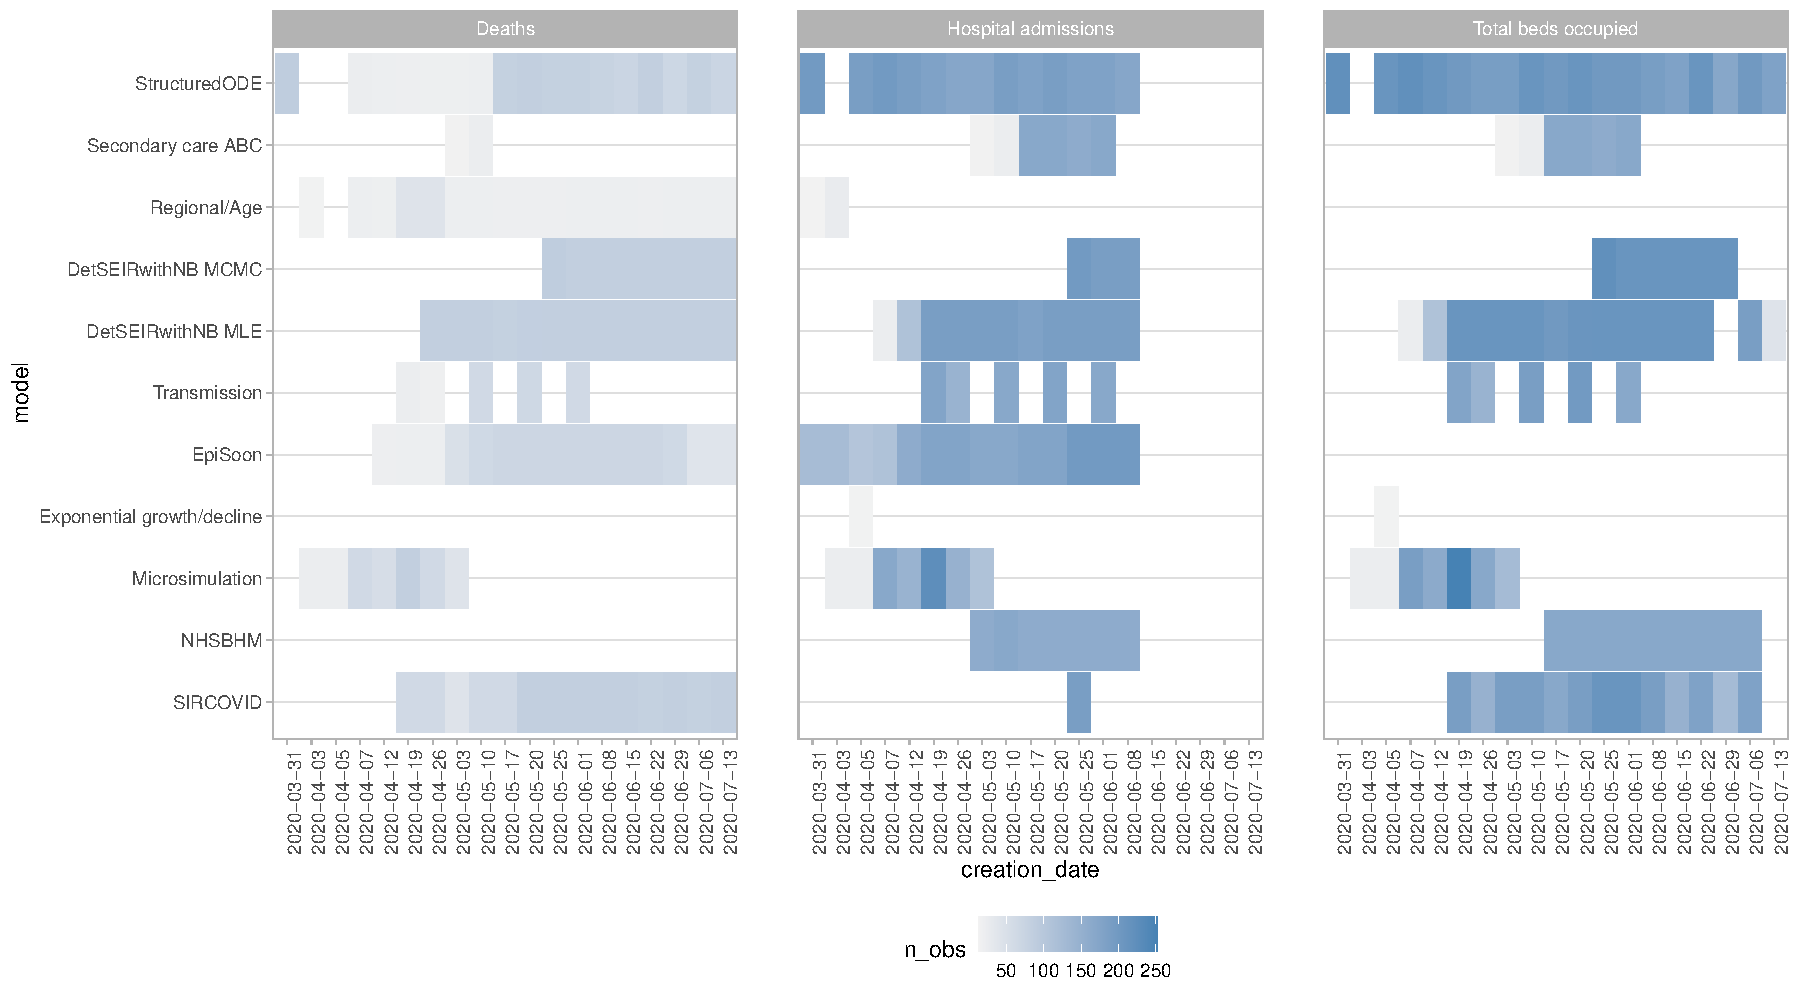
\includegraphics[width=\maxwidth]{plots/plot-show-availability-1} 
\end{knitrout}
\caption{\label{fig:avail-forecasts} Overview of the number of available forecasts}
\end{figure}
%THINK ABOUT WHETHER THIS FUNCTION CAN BE COMBINED WITH THE OTHER HEATMAP FUNCTION. 
% 
The forecasts and observed values themselves can be visualised using the \fct{plot\_predictions} function. Data visualisation is of course highly context-dependent, but the function tries to accommodate most practical use-cases. In addition to basic plotting functionality it offers the user an optional ad hoc way to filter both forecasts and observed values. This makes it possible to tweak the plot in a beginner-friendly way without having to manipulate the data separately. Forecasts and observed values can be passed in separately (and are merged internally) or as a single data.frame. Conditions to filter on need to be provided as a list of strings, where each of the strings represents an expression that can be evaluated to filter the data. To display, for example, short-term forecasts for COVID-19 cases and deaths made by the EuroCOVIDhub-ensemble model on June 28 2021 as well as 5 weeks of prior data, we can call: % 
\begin{figure}[h!]
\centering
\begin{knitrout}
\definecolor{shadecolor}{rgb}{0.969, 0.969, 0.969}\color{fgcolor}\begin{kframe}
\begin{alltt}
\hlstd{> }\hlkwd{plot_predictions}\hlstd{(}\hlkwc{data} \hlstd{= example_quantile,} \hlkwc{x} \hlstd{=} \hlstr{"target_end_date"}\hlstd{,}
\hlstd{+ }    \hlkwc{filter_truth} \hlstd{=} \hlkwd{list}\hlstd{(}\hlstr{"target_end_date <= \textbackslash{}"2021-07-15\textbackslash{}""}\hlstd{,}
\hlstd{+ }        \hlstr{"target_end_date > \textbackslash{}"2021-05-22\textbackslash{}""}\hlstd{),} \hlkwc{filter_forecasts} \hlstd{=} \hlkwd{list}\hlstd{(}\hlstr{"model == 'EuroCOVIDhub-ensemble'"}\hlstd{,}
\hlstd{+ }        \hlstr{"forecast_date == \textbackslash{}"2021-06-28\textbackslash{}""}\hlstd{),} \hlkwc{facet_formula} \hlstd{= target_type} \hlopt{~}
\hlstd{+ }        \hlstd{location,} \hlkwc{ncol} \hlstd{=} \hlnum{4}\hlstd{)} \hlopt{+} \hlstd{ggplot2}\hlopt{::}\hlkwd{theme}\hlstd{(}\hlkwc{legend.position} \hlstd{=} \hlstr{"bottom"}\hlstd{)}
\end{alltt}
\end{kframe}
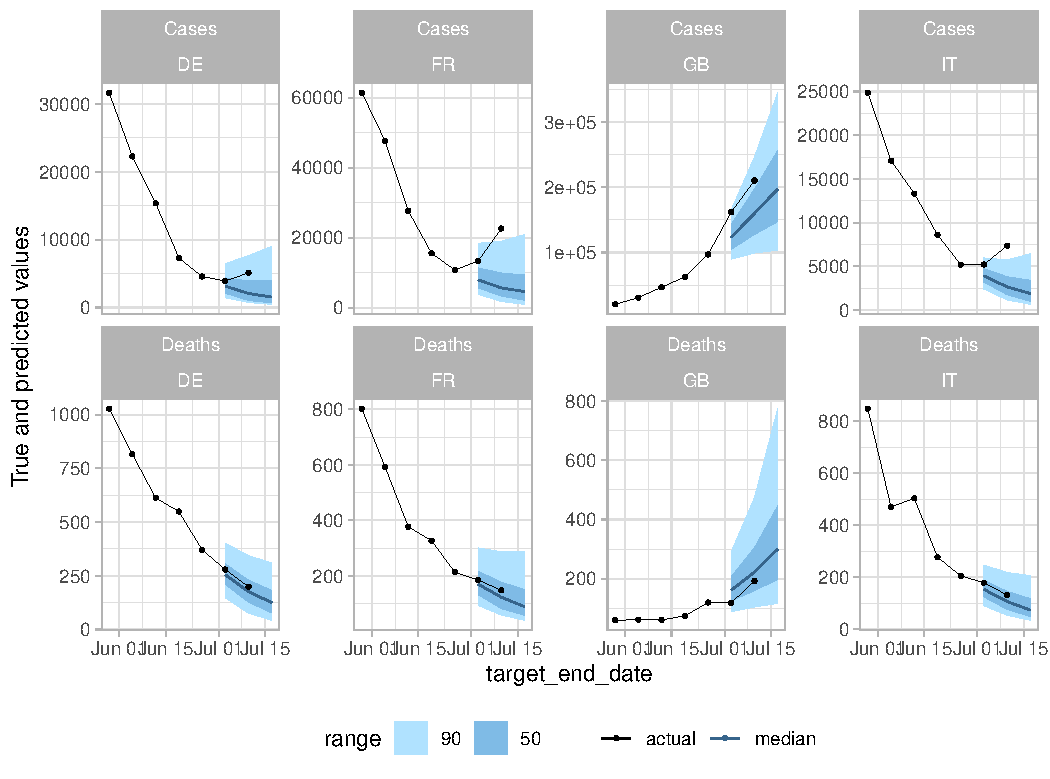
\includegraphics[width=\maxwidth]{plots/plot-show-forecasts-1} 
\end{knitrout}
\caption{\label{fig:forecast-visualisation} Short-term forecasts for COVID-19 cases and deaths made by the EuroCOVIDhub-ensemble model on June 28 2021.}
\end{figure}
% 
The output is shown in Figure \ref{fig:forecast-visualisation}.

\subsection[Scoring forecasts and obtaining a model ranking]{Scoring forecasts with \fct{eval\_forecasts}}

The actual scoring of forecasts based on observed values can be performed using the function \fct{eval\_forecasts}. The function automatically detects the forecast type and format (as shown in the output of \fct{check\_forecasts}), applies the appropriate scoring metrics and can in addition also aggregate results as well as perform pairwise comparisons between models. Internally, operations are handled using \pkg{data.table} to allow for fast and efficient computation. 

\begin{knitrout}
\definecolor{shadecolor}{rgb}{0.969, 0.969, 0.969}\color{fgcolor}\begin{kframe}
\begin{alltt}
\hlstd{> }\hlstd{scores} \hlkwb{<-} \hlkwd{eval_forecasts}\hlstd{(example_quantile)}
\hlstd{> }\hlkwd{glimpse}\hlstd{(scores)}
\end{alltt}
\begin{verbatim}
## Rows: 887
## Columns: 14
## $ location           <chr> "DE", "DE", "DE", "DE", "DE", "DE", "DE", "DE", "DE~
## $ target_end_date    <date> 2021-05-08, 2021-05-08, 2021-05-08, 2021-05-08, 20~
## $ target_type        <chr> "Cases", "Cases", "Cases", "Deaths", "Deaths", "Dea~
## $ location_name      <chr> "Germany", "Germany", "Germany", "Germany", "German~
## $ forecast_date      <chr> "2021-05-03", "2021-05-03", "2021-05-03", "2021-05-~
## $ model              <chr> "EuroCOVIDhub-baseline", "EuroCOVIDhub-ensemble", "~
## $ horizon            <dbl> 1, 1, 1, 1, 1, 1, 1, 2, 2, 2, 1, 1, 1, 2, 2, 2, 2, ~
## $ interval_score     <dbl> 16925.04696, 7990.85478, 25395.96087, 46.79304, 53.~
## $ dispersion         <dbl> 1649.22087, 5440.98522, 8173.70000, 44.66261, 53.27~
## $ underprediction    <dbl> 0.0000000, 0.0000000, 0.0000000, 0.0000000, 0.60869~
## $ overprediction     <dbl> 15275.826087, 2549.869565, 17222.260870, 2.130435, ~
## $ coverage_deviation <dbl> -0.38521739, 0.04956522, -0.29826087, 0.22347826, 0~
## $ bias               <dbl> 0.95, 0.50, 0.90, 0.30, -0.10, -0.50, 0.10, 1.00, 0~
## $ aem                <dbl> 25620, 12271, 44192, 15, 14, 208, 24, 67622, 45731,~
\end{verbatim}
\end{kframe}
\end{knitrout}

The above produces one score for every forecast. However, we usually like to summarise scores to learn about average performance. 

We can either run a separate function to summarise the scores, 
\begin{knitrout}
\definecolor{shadecolor}{rgb}{0.969, 0.969, 0.969}\color{fgcolor}\begin{kframe}
\begin{alltt}
\hlstd{> }\hlstd{summarised_scores} \hlkwb{<-} \hlkwd{summarise_scores}\hlstd{(}\hlkwc{scores} \hlstd{= scores,} \hlkwc{summarise_by} \hlstd{=} \hlkwd{c}\hlstd{(}\hlstr{"model"}\hlstd{,}
\hlstd{+ }    \hlstr{"target_type"}\hlstd{))}
\end{alltt}
\end{kframe}
\end{knitrout}

or we score and summarise in one function call: 

\begin{knitrout}
\definecolor{shadecolor}{rgb}{0.969, 0.969, 0.969}\color{fgcolor}\begin{kframe}
\begin{alltt}
\hlstd{> }\hlstd{summarised_scores} \hlkwb{<-} \hlkwd{eval_forecasts}\hlstd{(example_quantile,} \hlkwc{summarise_by} \hlstd{=} \hlkwd{c}\hlstd{(}\hlstr{"model"}\hlstd{,}
\hlstd{+ }    \hlstr{"target_type"}\hlstd{))}
\end{alltt}
\end{kframe}
\end{knitrout}

\begin{knitrout}
\definecolor{shadecolor}{rgb}{0.969, 0.969, 0.969}\color{fgcolor}\begin{kframe}
\begin{alltt}
\hlstd{> }\hlstd{summarised_scores}
\end{alltt}
\begin{verbatim}
##                    model target_type interval_score dispersion underprediction
## 1: EuroCOVIDhub-baseline       Cases    28483.57465 4102.50094    10284.972826
## 2: EuroCOVIDhub-ensemble       Cases    17943.82383 3663.52458     4237.177310
## 3:  epiforecasts-EpiNow2       Cases    20831.55662 5664.37795     3260.355639
## 4: EuroCOVIDhub-baseline      Deaths      159.40387   91.40625        2.098505
## 5: EuroCOVIDhub-ensemble      Deaths       41.42249   30.18099        4.103261
## 6:       UMass-MechBayes      Deaths       52.65195   26.87239       16.800951
## 7:  epiforecasts-EpiNow2      Deaths       66.64282   31.85692       15.893314
##    overprediction coverage_deviation        bias         aem
## 1:   14096.100883        -0.11211957  0.09796875 38473.60156
## 2:   10043.121943        -0.09785326 -0.05640625 24101.07031
## 3:   11906.823030        -0.06660326 -0.07890625 27923.81250
## 4:      65.899117         0.11614130  0.33906250   233.25781
## 5:       7.138247         0.19528533  0.07265625    53.13281
## 6:       8.978601        -0.02312500 -0.02234375    78.47656
## 7:      18.892583        -0.04287176 -0.00512605   104.74790
\end{verbatim}
\end{kframe}
\end{knitrout}


% 
\fct{eval\_forecasts} and \fct{summarise\_scores} aggregate scores by taking the mean over according to the grouping specified in \code{summarise_by}. In the above example, if \code{summarise_by = c("model", "target_type")}, then scores would be averaged over all other categories to obtain one score per model and forecast target type. For a more detailed analysis we could for example specify \code{summarise_by = c("mode", "target_type", "location")} to additionally stratify by country. Summarised scores can be visualised using the function \fct{scores\_table} as is shown in Figure \ref{fig:score-table}. 

If we wanted to have one score per quantile or one per prediction interval range, we could use something like \code{summarise_by = c("model", "quantile", "range")}. This would allow us to examine interval or quantile coverage or makes it possible to analyse the accuracy of the tails of the forecasts. In addition to the mean, we can also obtain the standard deviation of the scores over which we average, as well as any desired quantile, by specifying \code{sd = TRUE} and for example \code{quantiles = c(0.5)} for the median. 

The user must, however, exercise some caution when aggregating scores. As explained above, many of the metrics are absolute and scale with the magnitude of the quantity to forecast. This makes it sometimes ill-advised to average over them. In the given example, looking at one score per model (i.e. specifying \code{summarise_by = c("model")}) is problematic, as overall aggregate scores would be dominated by case forecasts, while errors on death forecasts would have little influence. Similarly, aggregating over different forecast horizons is often not a good idea as the mean will be dominated by further ahead forecast horizons. 

\begin{figure}[h]
\centering
\begin{knitrout}
\definecolor{shadecolor}{rgb}{0.969, 0.969, 0.969}\color{fgcolor}\begin{kframe}
\begin{alltt}
\hlstd{> }\hlkwd{score_table}\hlstd{(summarised_scores,} \hlkwc{y} \hlstd{=} \hlstr{"model"}\hlstd{,} \hlkwc{facet_formula} \hlstd{=} \hlopt{~}\hlstd{target_type)}
\end{alltt}
\end{kframe}
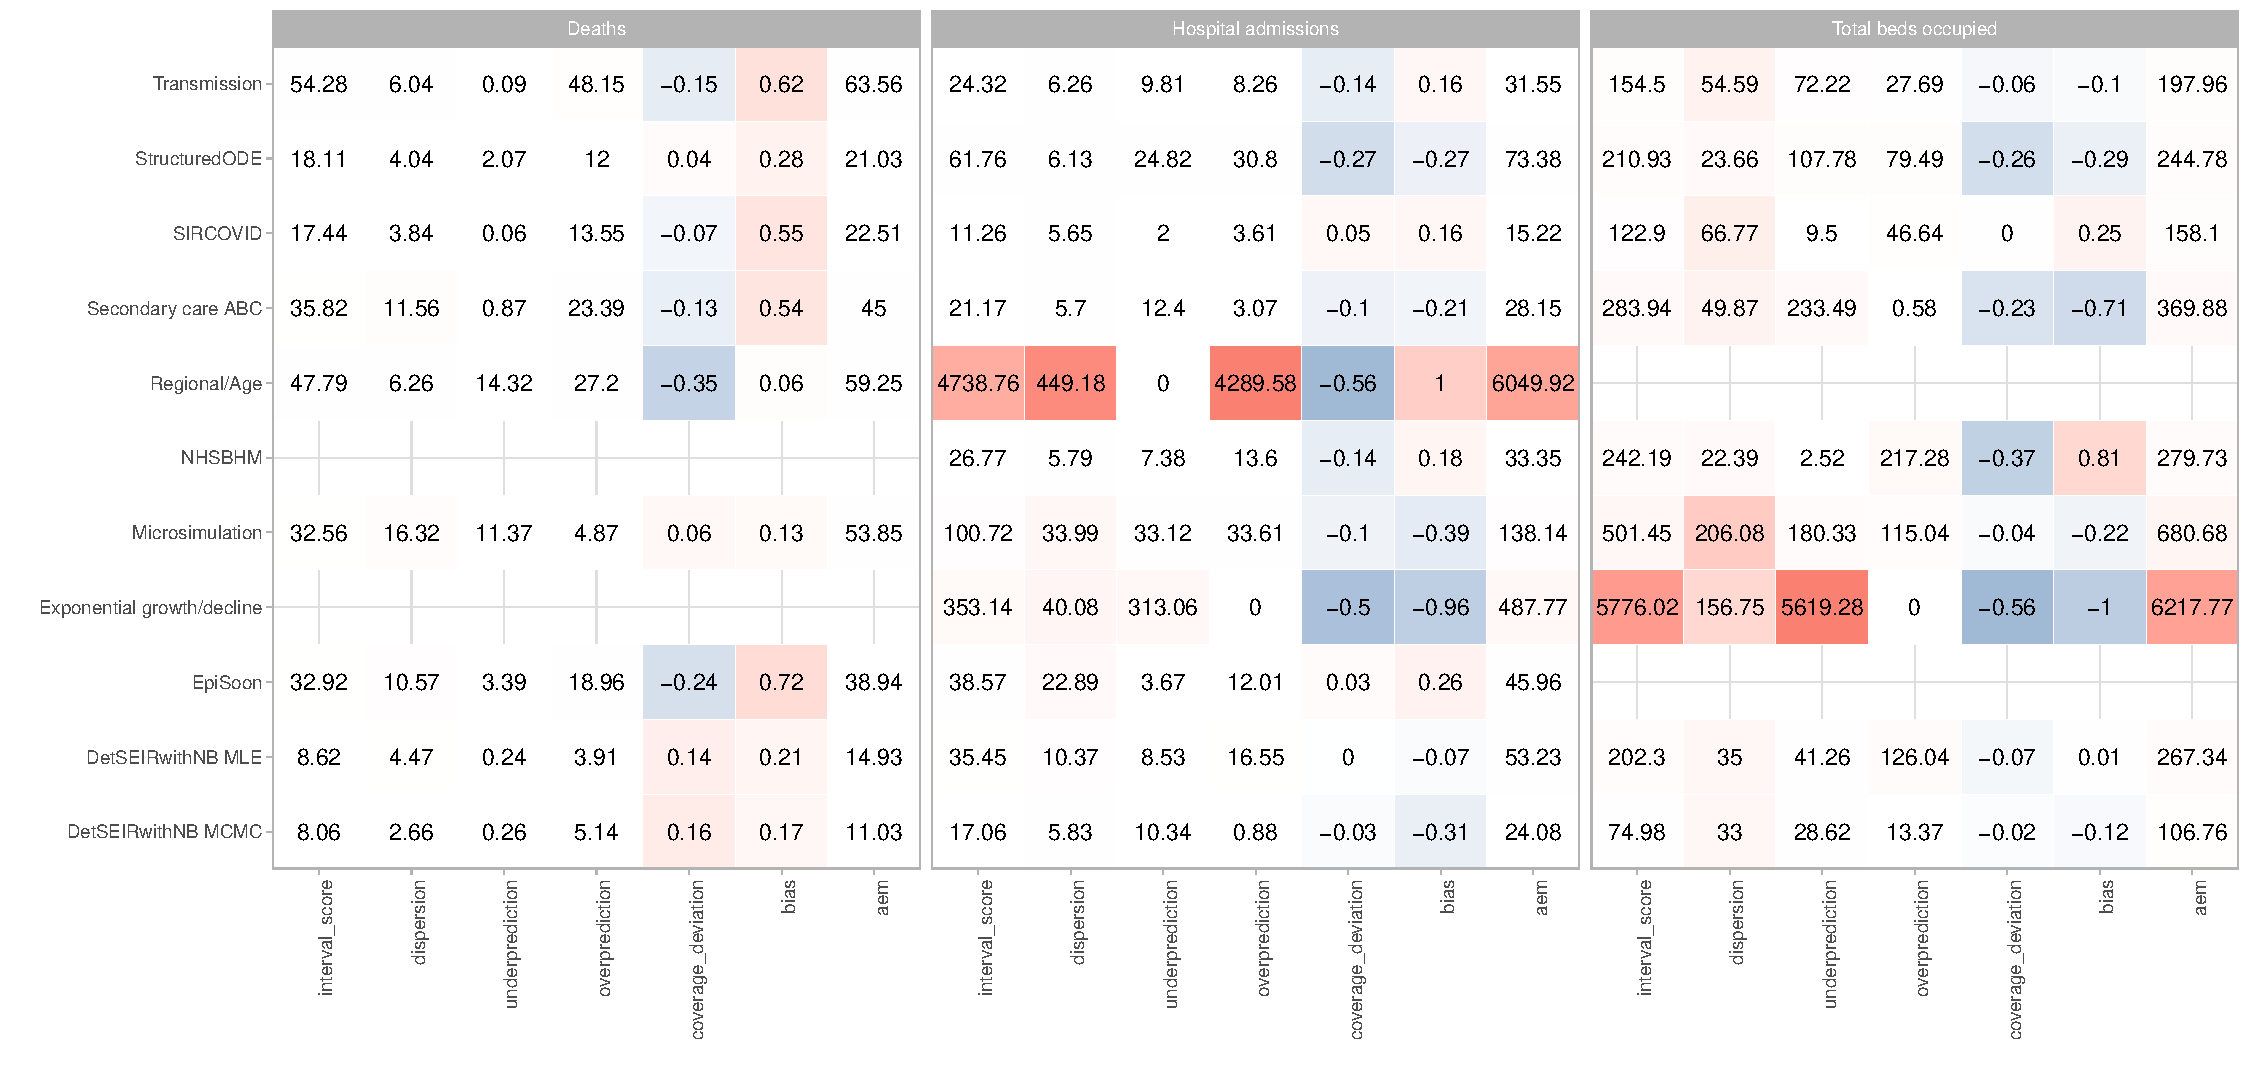
\includegraphics[width=\maxwidth]{plots/plot-score-table-1} 
\end{knitrout}
\caption{\label{fig:score-table} Coloured table to visualise the computed scores}
\end{figure}

In order to obtain a model ranking, we recommend to look at the relative skill in terms of an appropriate proper scoring rule instead of the raw score. Relative skill scores can be aggregated more easily across different forecast targets as they are less influenced by the order of magnitude of the quantity to forecast than e.g. the WIS or the CRPS. 

Again there are two possible ways to do pairwise comparisons. First, the function \fct{pairiwse\_comparison} can be called to compare models against each other. Here \code{summarise_by} denotes what relative skill scores shall be computed for. \code{summarise_by = "model"} means there will be one relative skill score per model, while \code{summarise_by = c("target_type", "target_type")} would mean there is one relative skill score per model, computed completely separately for different target types. 

When using \fct{pairwise\_comparison}, it is important that the scores used as input have not been summarised in any way. 

\begin{knitrout}
\definecolor{shadecolor}{rgb}{0.969, 0.969, 0.969}\color{fgcolor}\begin{kframe}
\begin{alltt}
\hlstd{> }\hlstd{pairwise} \hlkwb{<-} \hlkwd{pairwise_comparison}\hlstd{(scores,} \hlkwc{baseline} \hlstd{=} \hlstr{"EuroCOVIDhub-baseline"}\hlstd{)}
\hlstd{> }
\hlstd{> }\hlstd{pairwise2} \hlkwb{<-} \hlkwd{pairwise_comparison}\hlstd{(scores,} \hlkwc{summarise_by} \hlstd{=} \hlkwd{c}\hlstd{(}\hlstr{"model"}\hlstd{,}
\hlstd{+ }    \hlstr{"target_type"}\hlstd{),} \hlkwc{baseline} \hlstd{=} \hlstr{"EuroCOVIDhub-baseline"}\hlstd{)}
\end{alltt}
\end{kframe}
\end{knitrout}

Pairwise comparisons between models [CITATION] can be obtained in two different ways. First, relative skill scores based on pairwise comparisons are by default returned from \fct{eval\_forecasts}. These will be computed separately for the categories defined in the \code{summarise_by} argument (excluding the category 'model'). Alternatively, a set of scores can be post-processed using the separate function \fct{pairwise\_comparison}. This approach is to be used for visualisation and if p-values for the pairwise comparisons are needed, as those are not returned from \fct{eval\_forecasts}. Usually, one would compute scores without specifying a \code{summarise_by} argument, but sometimes it may be sensible to average over certain scores, for example for predictions generated at a certain date. This allows to reduce the correlation between observations that enter the computation of p-values, which in turn makes the test less liberal. 
Using the function \fct{plot\_pairwise\_comparison} we can visualise the mean score ratios between all models as well as the 

The result is a \code{data.table} with different scores and metrics in a tidy format that can easily be used for further manipulation and plotting. 

\begin{figure}[h!]
\centering
\begin{knitrout}
\definecolor{shadecolor}{rgb}{0.969, 0.969, 0.969}\color{fgcolor}\begin{kframe}
\begin{alltt}
\hlstd{> }\hlkwd{plot_pairwise_comparison}\hlstd{(pairwise2)} \hlopt{+} \hlstd{ggplot2}\hlopt{::}\hlkwd{facet_wrap}\hlstd{(}\hlopt{~}\hlstd{target_type,}
\hlstd{+ }    \hlkwc{scales} \hlstd{=} \hlstr{"free_x"}\hlstd{)}
\end{alltt}
\end{kframe}
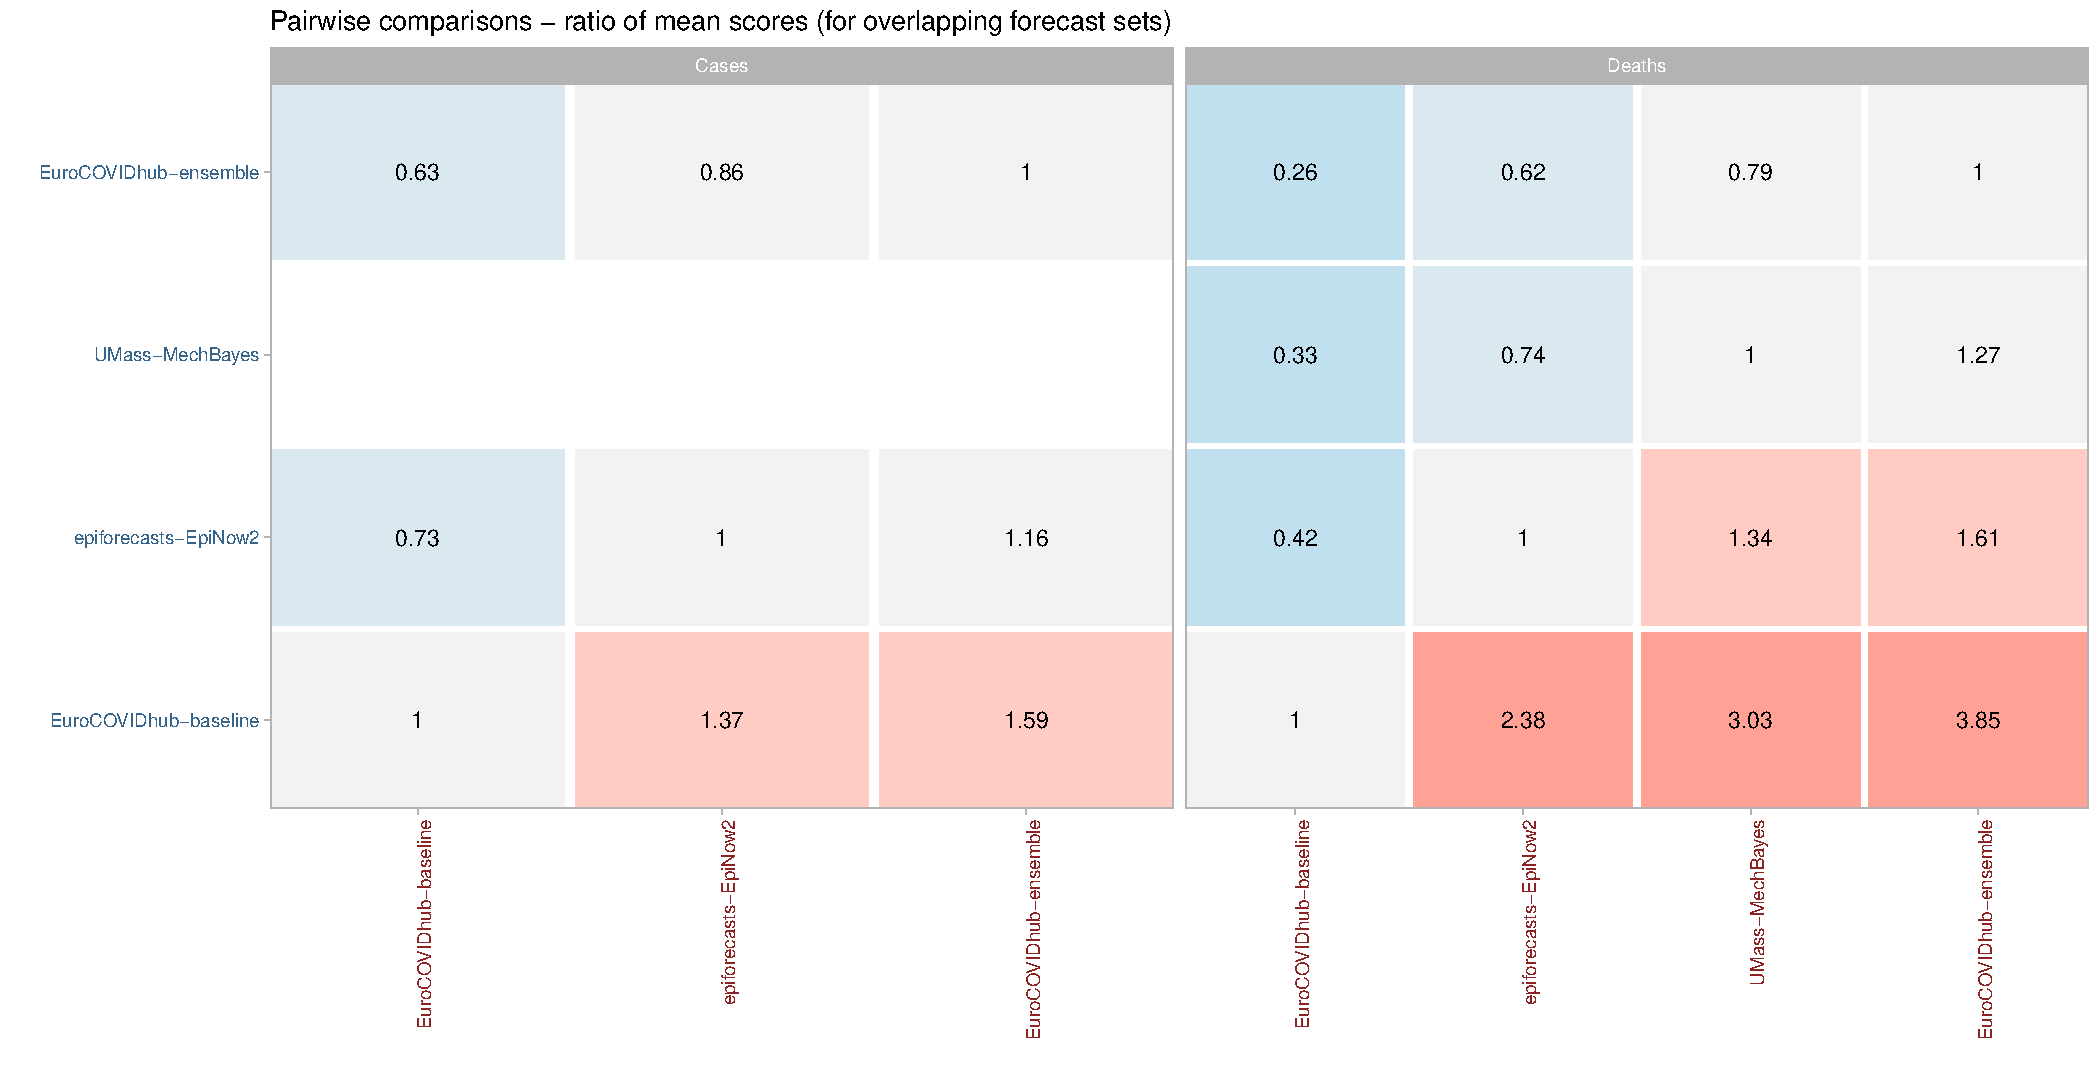
\includegraphics[width=\maxwidth]{plots/plot-pairwise-plot-1} 
\end{knitrout}
\caption{\label{fig:pairwise-comparison} Ratios of mean scores based on overlapping forecast sets. If a tile is blue, then the model on the y-axis performed better. If it is red, the model on the x-axis performed better in direct comparison. }
\end{figure}

\section{Visualisation and interpretation of evaluation results}

\subsection{Visualising aggregate scores and rankings}
A good starting point for an evaluation is the following score table that visusalises the scores we produced above. We can facet the table to account for the different forecast targets: 


The most informative metric in terms of model ranking is the relative\_skill. However, interpretation is not always straightforward and has to be done carefully. We can see that performance varied quite a bit across different metrics, where some models did well on one target, but poorly on another. Especially the Exponential growth/decline model stands out as it received the lowest relative skill score for hospital admissions, but the highest for the total number of beds occupied. Looking back at Figure \ref{fig:avail-forecasts}, we see that the model has only submitted very few forecasts over all. It may therefore be sensible to require all models to have submitted forecasts for at least 50\% of all forecast targets in order to enter the pairwise comparisons. For similar reasons, the interval score may be deceiving if looked at in isolation. As can be seen, the DetSEIRwithNB MLE model received a lower relative skill score, but a higher interval score than the DetSEIRwithNB MCMC model. This, again, can be explained by the fact that they forecasted different targets. The interval score, as an absolute metric, is highly influenced by the absolute value of the quantity that is forecasted. For the same reason, one should be careful when summarising interval scores from different locations or forecast targets, as the average score will be dominated by outliers as well as differences in the absolute level. Assuming a large enough set of available overlapping forecasts, the relative skill score is more robust. It therefore is reasonable to assume that the DetSEIRwithNB MLE forecasted quantities with a higher absolute value, but tended to perform worse than the DetSEIRwithNB MCMC model as far as we can tell based on the set of all pariwise comparisons. This can be confirmed for the direct comparison between the two by looking at the mean score ratios from the pairwise comparisons. These can be obtained by calling

In terms of actually understanding \textit{why} one model performs well or badly, the other metrics shown in Figure \ref{fig:score-table} provide additional insight. We turn to them in the following. 

\subsection{Visual model diagnostics}

For forecasts in an interval format, looking at the components of the weighted interval score separately is a natural next step. We can see in Figure \ref{fig:wis-components} that the majority of penalties come from over-and underprediction, instead of the sharpness component. We also see that most models tended to either over- or underpredict actual numbers.  

\begin{figure}[h!]
\centering
\begin{knitrout}
\definecolor{shadecolor}{rgb}{0.969, 0.969, 0.969}\color{fgcolor}\begin{kframe}
\begin{alltt}
\hlstd{> }\hlkwd{wis_components}\hlstd{(summarised_scores,} \hlkwc{facet_formula} \hlstd{=} \hlopt{~}\hlstd{target_type,}
\hlstd{+ }    \hlkwc{scales} \hlstd{=} \hlstr{"free_x"}\hlstd{,} \hlkwc{relative_contributions} \hlstd{=} \hlnum{TRUE}\hlstd{,} \hlkwc{x_text_angle} \hlstd{=} \hlnum{0}\hlstd{)} \hlopt{+}
\hlstd{+ }    \hlstd{ggplot2}\hlopt{::}\hlkwd{coord_flip}\hlstd{()} \hlopt{+} \hlstd{ggplot2}\hlopt{::}\hlkwd{theme}\hlstd{(}\hlkwc{legend.position} \hlstd{=} \hlstr{"bottom"}\hlstd{)}
\end{alltt}
\end{kframe}
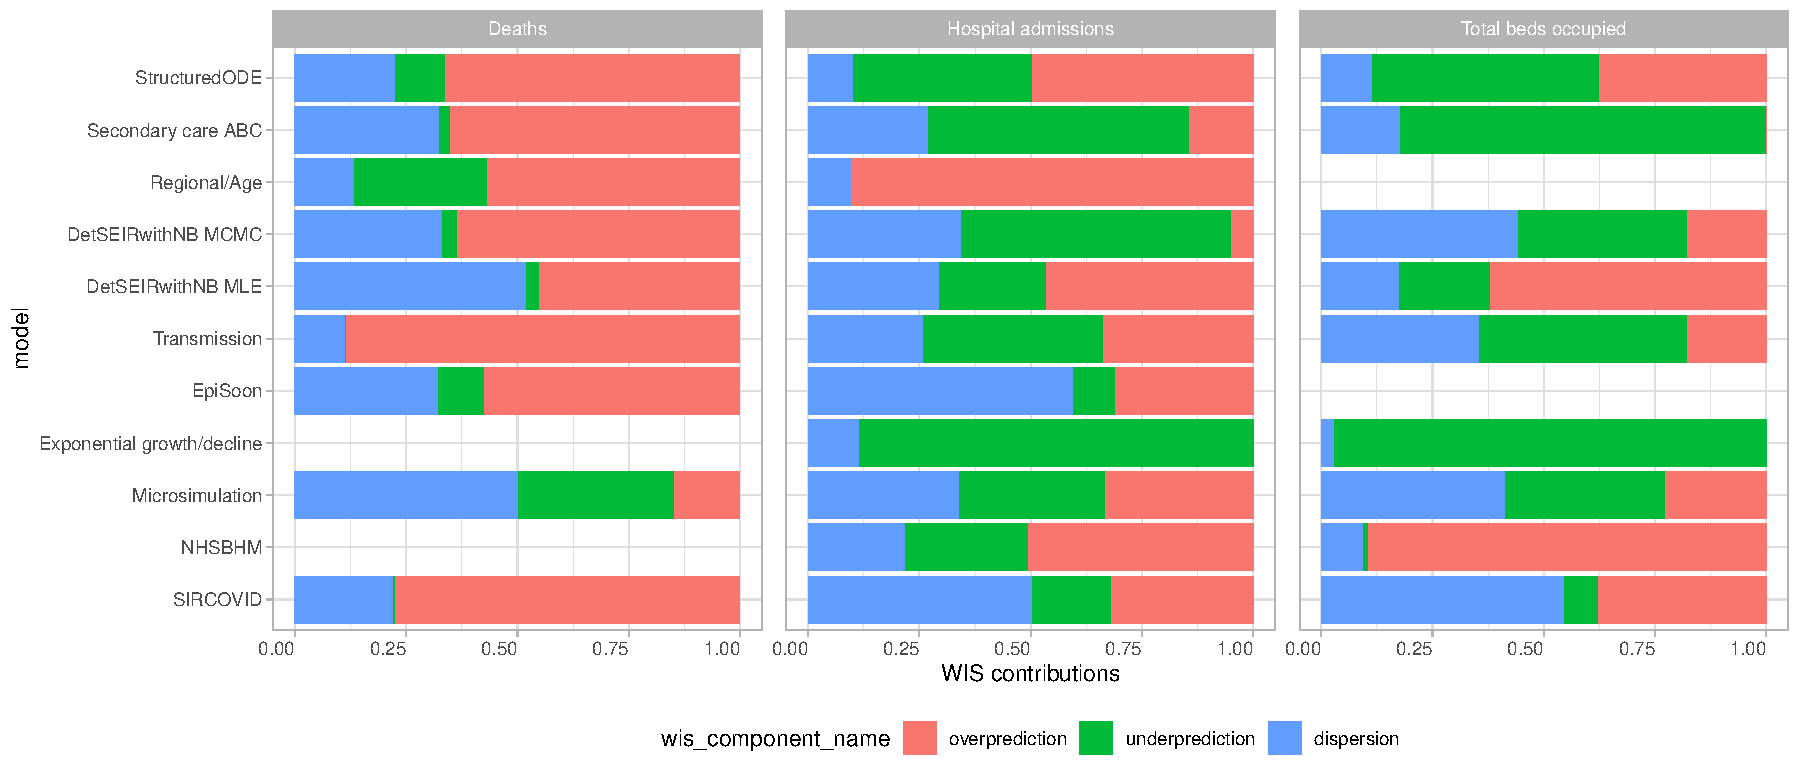
\includegraphics[width=\maxwidth]{plots/plot-WIS-components-1} 
\end{knitrout}
\caption{\label{fig:wis-components} p-values and ratios together.}
\end{figure}

We can have a closer look at calibration using the functions \fct{interval\_coverage} and \fct{quantile\_coverage}. The interval coverage plot shows the proportion of all true values that fall within all the different prediction intervals. This gives a visual impression of probabilistic calibration \ref{gneitingProbabilisticForecastsCalibration2007}. Ideally, $x$ percent of true values should be covered by the $x$\%-prediction intervals, resulting in a 45° line. Areas shaded in green indicate that the model is covering more true values than it actually should, while areas in white indicate that the model fails to cover the desired proportion of true values with its prediction intervals. The majority of the models were too confident in their predictions, while some showed showed good calibration. The quantile coverage plot shows the proportion of all true values below certain predictive quantiles. While this plot is slightly harder to interpret, it also includes information about bias as and allows to separate the lower and upper boundaries of the prediction intervals. We can see, for example, that the Exponential growth/decline model was consistently biased downwards. Figure \ref{fig:coverage}

\begin{knitrout}
\definecolor{shadecolor}{rgb}{0.969, 0.969, 0.969}\color{fgcolor}\begin{kframe}
\begin{alltt}
\hlstd{> }\hlstd{pit} \hlkwb{<-} \hlkwd{pit_df}\hlstd{(example_quantile,} \hlkwc{summarise_by} \hlstd{=} \hlstr{"model"}\hlstd{,} \hlstr{"target"}\hlstd{)}
\hlstd{> }
\hlstd{> }\hlkwd{hist_PIT}\hlstd{(pit)}
\end{alltt}
\begin{verbatim}
## $`EuroCOVIDhub-baseline`
## 
## $`EuroCOVIDhub-ensemble`
## 
## $`epiforecasts-EpiNow2`
## 
## $`UMass-MechBayes`
\end{verbatim}
\end{kframe}

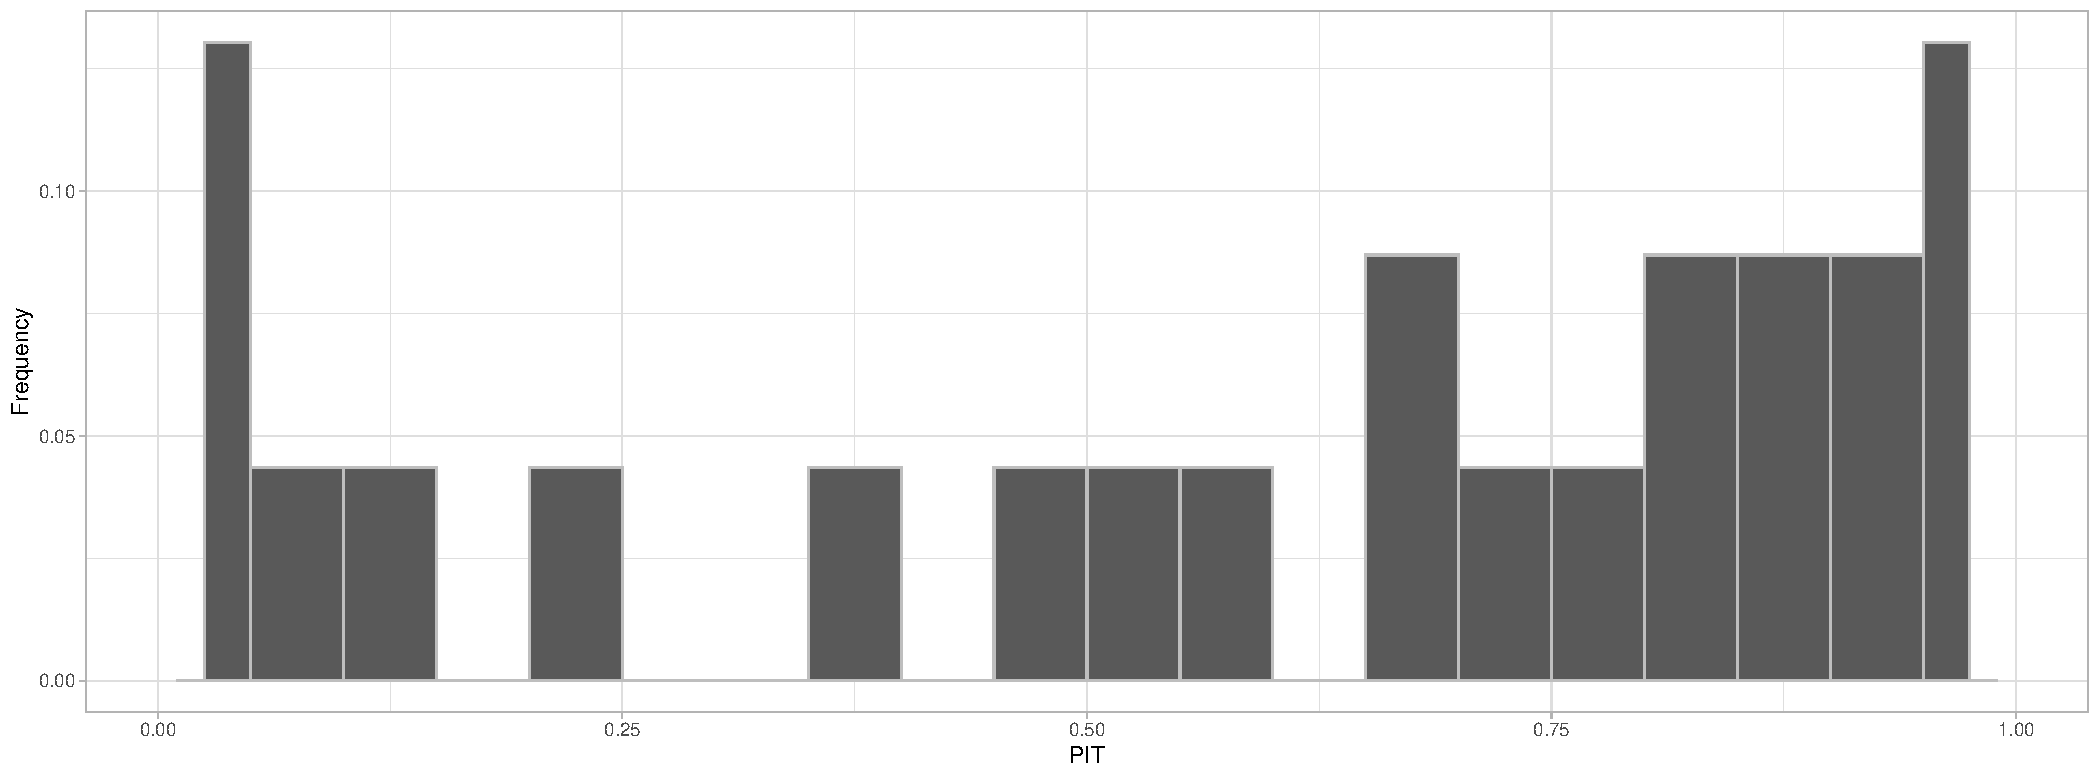
\includegraphics[width=0.49\linewidth]{plots/plot-pit-plots-1} 
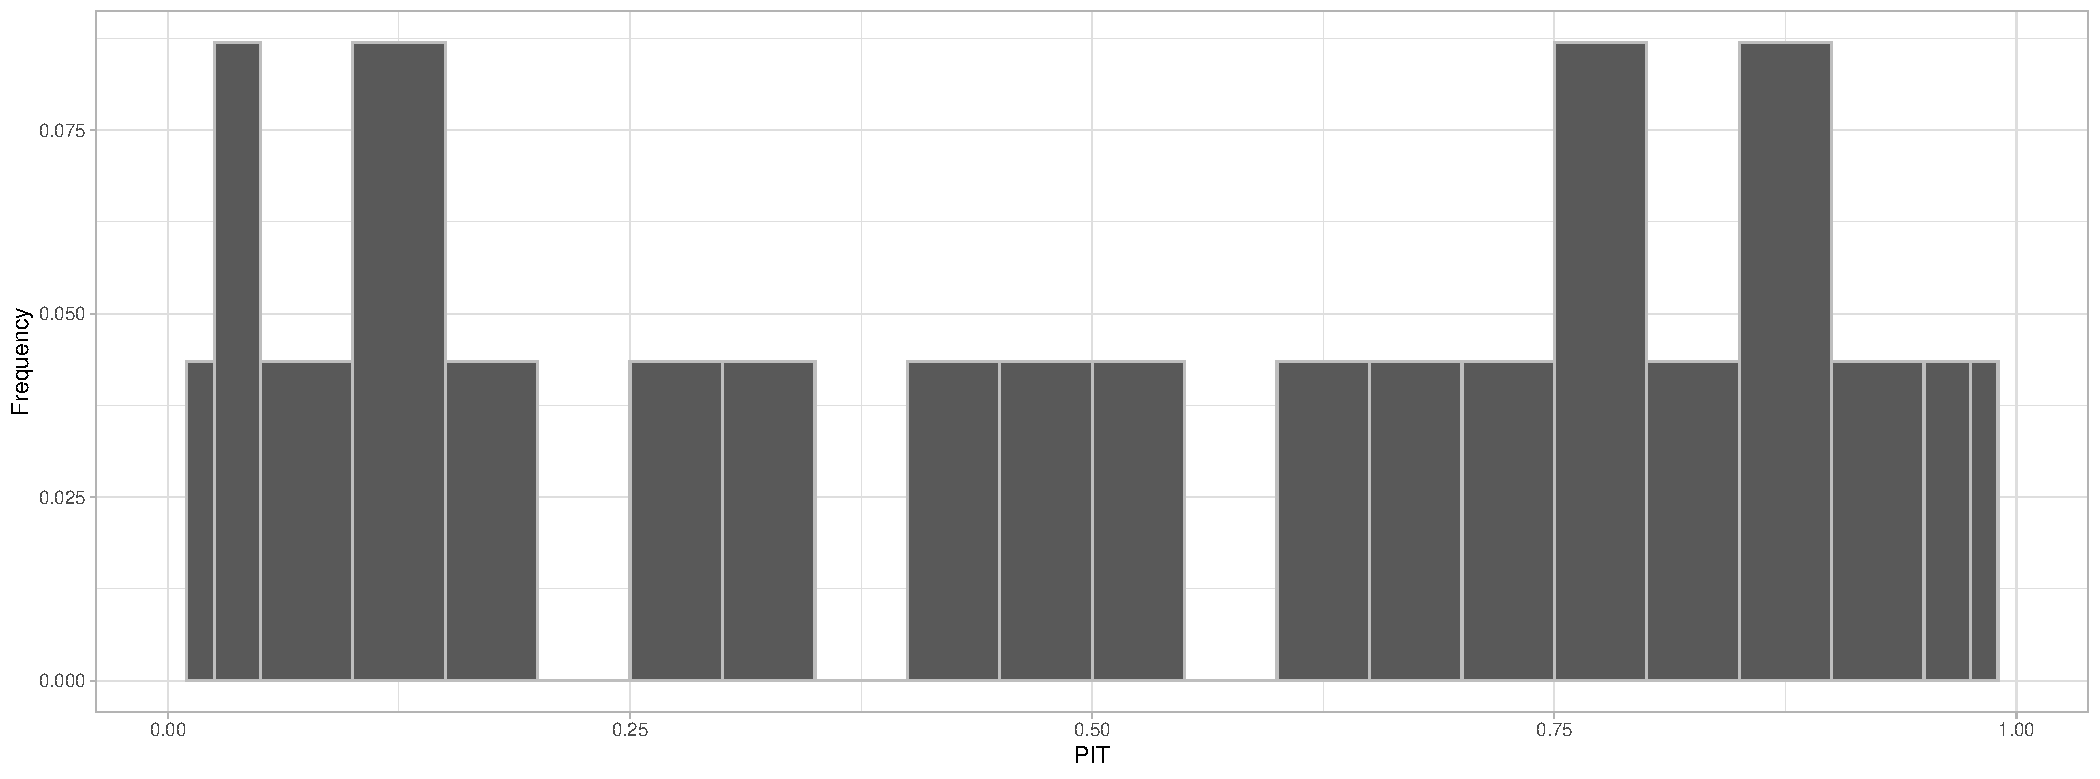
\includegraphics[width=0.49\linewidth]{plots/plot-pit-plots-2} 
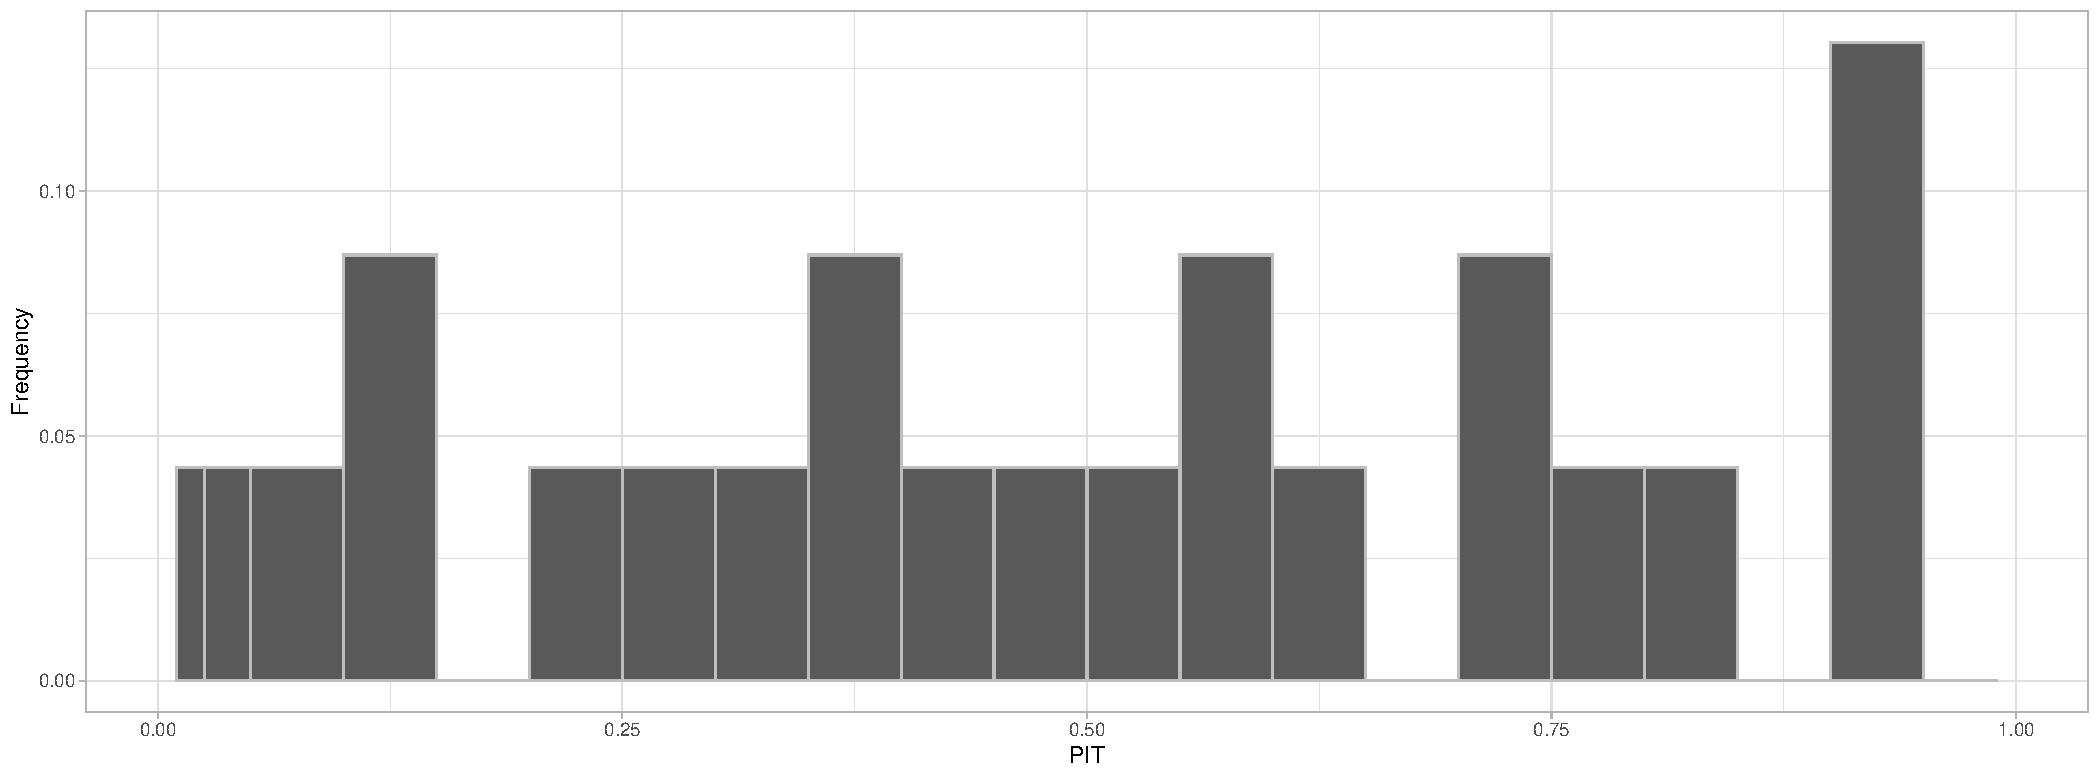
\includegraphics[width=0.49\linewidth]{plots/plot-pit-plots-3} 
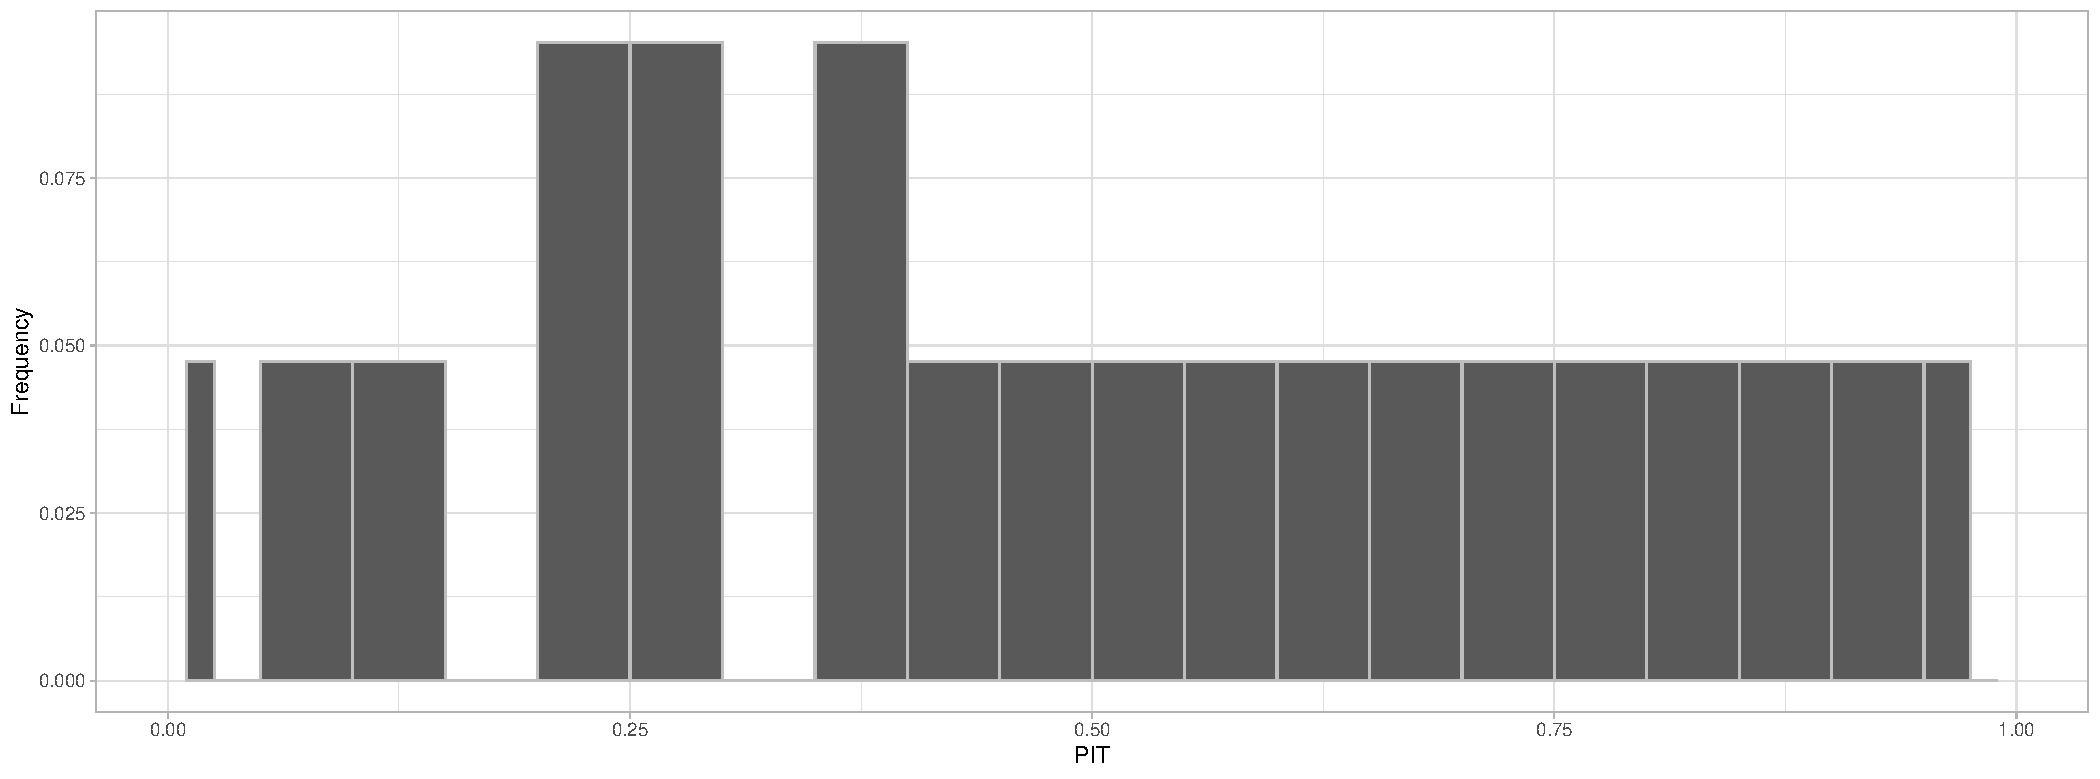
\includegraphics[width=0.49\linewidth]{plots/plot-pit-plots-4} 
\end{knitrout}



\begin{figure}[h!]
\centering
\begin{knitrout}
\definecolor{shadecolor}{rgb}{0.969, 0.969, 0.969}\color{fgcolor}\begin{kframe}
\begin{alltt}
\hlstd{> }\hlstd{cov_scores} \hlkwb{<-} \hlkwd{eval_forecasts}\hlstd{(example_quantile,} \hlkwc{summarise_by} \hlstd{=} \hlkwd{c}\hlstd{(}\hlstr{"model"}\hlstd{,}
\hlstd{+ }    \hlstr{"target_type"}\hlstd{,} \hlstr{"range"}\hlstd{,} \hlstr{"quantile"}\hlstd{))}
\hlstd{> }
\hlstd{> }\hlstd{scoringutils}\hlopt{::}\hlkwd{interval_coverage}\hlstd{(cov_scores,} \hlkwc{facet_formula} \hlstd{=} \hlopt{~}\hlstd{target_type)}
\end{alltt}
\end{kframe}
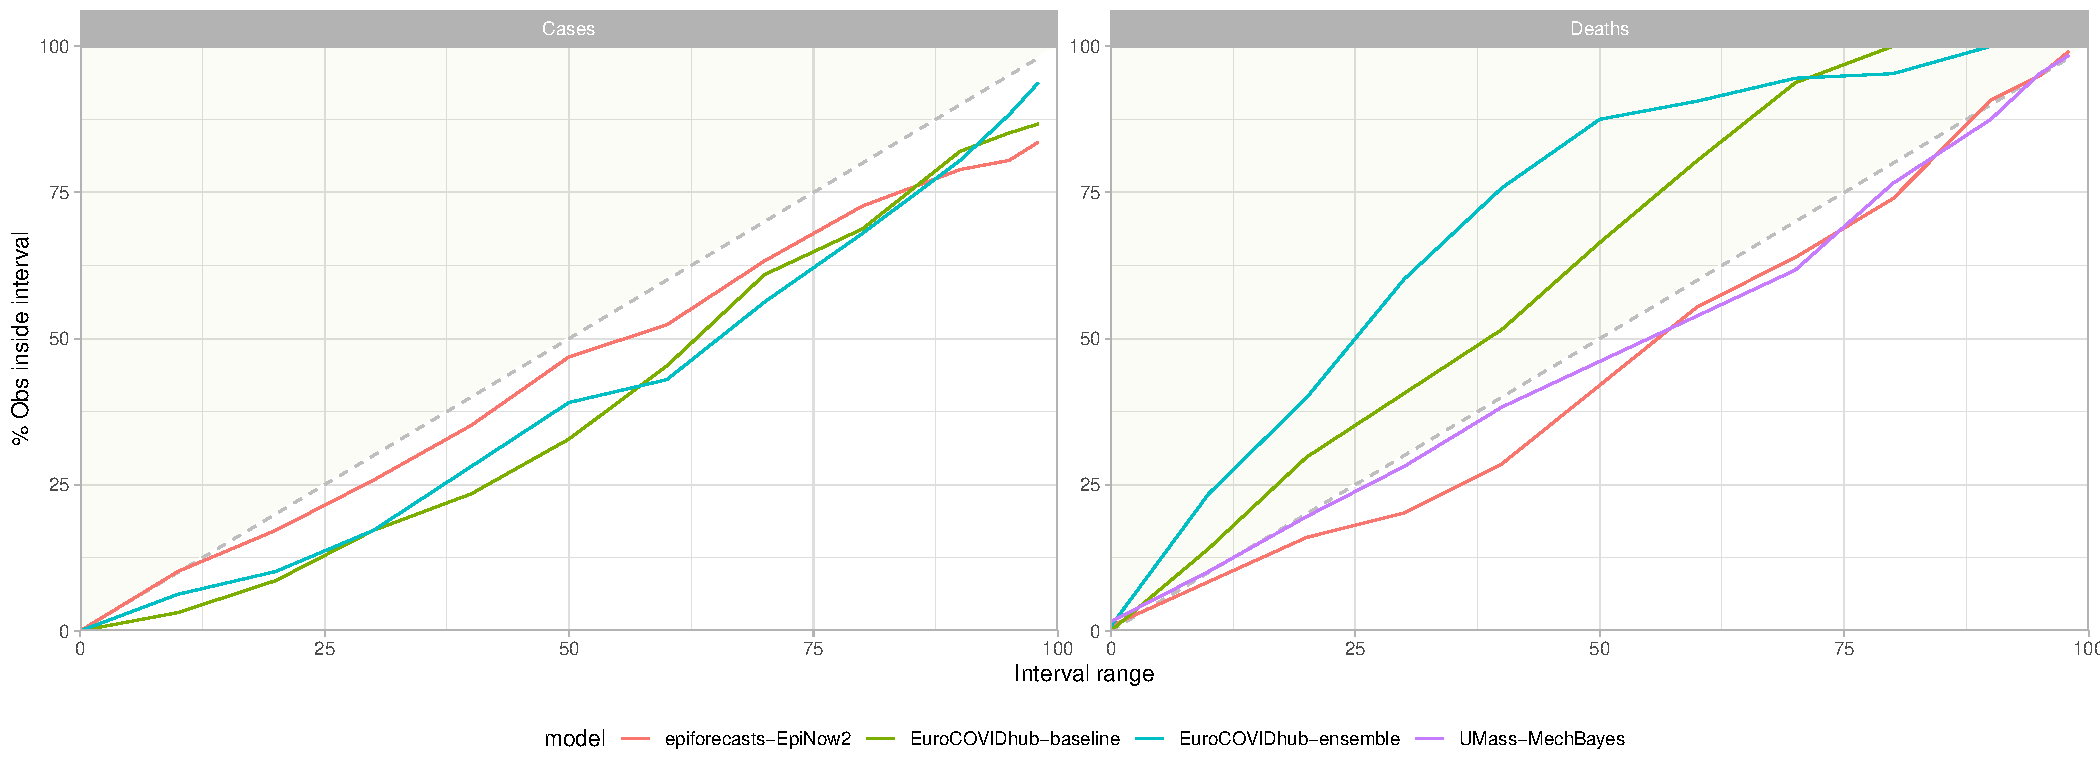
\includegraphics[width=\maxwidth]{plots/plot-coverage-1} 
\end{knitrout}


\begin{knitrout}
\definecolor{shadecolor}{rgb}{0.969, 0.969, 0.969}\color{fgcolor}\begin{kframe}
\begin{alltt}
\hlstd{> }\hlstd{scoringutils}\hlopt{::}\hlkwd{quantile_coverage}\hlstd{(cov_scores,} \hlkwc{facet_formula} \hlstd{=} \hlopt{~}\hlstd{target_type)}
\end{alltt}
\end{kframe}
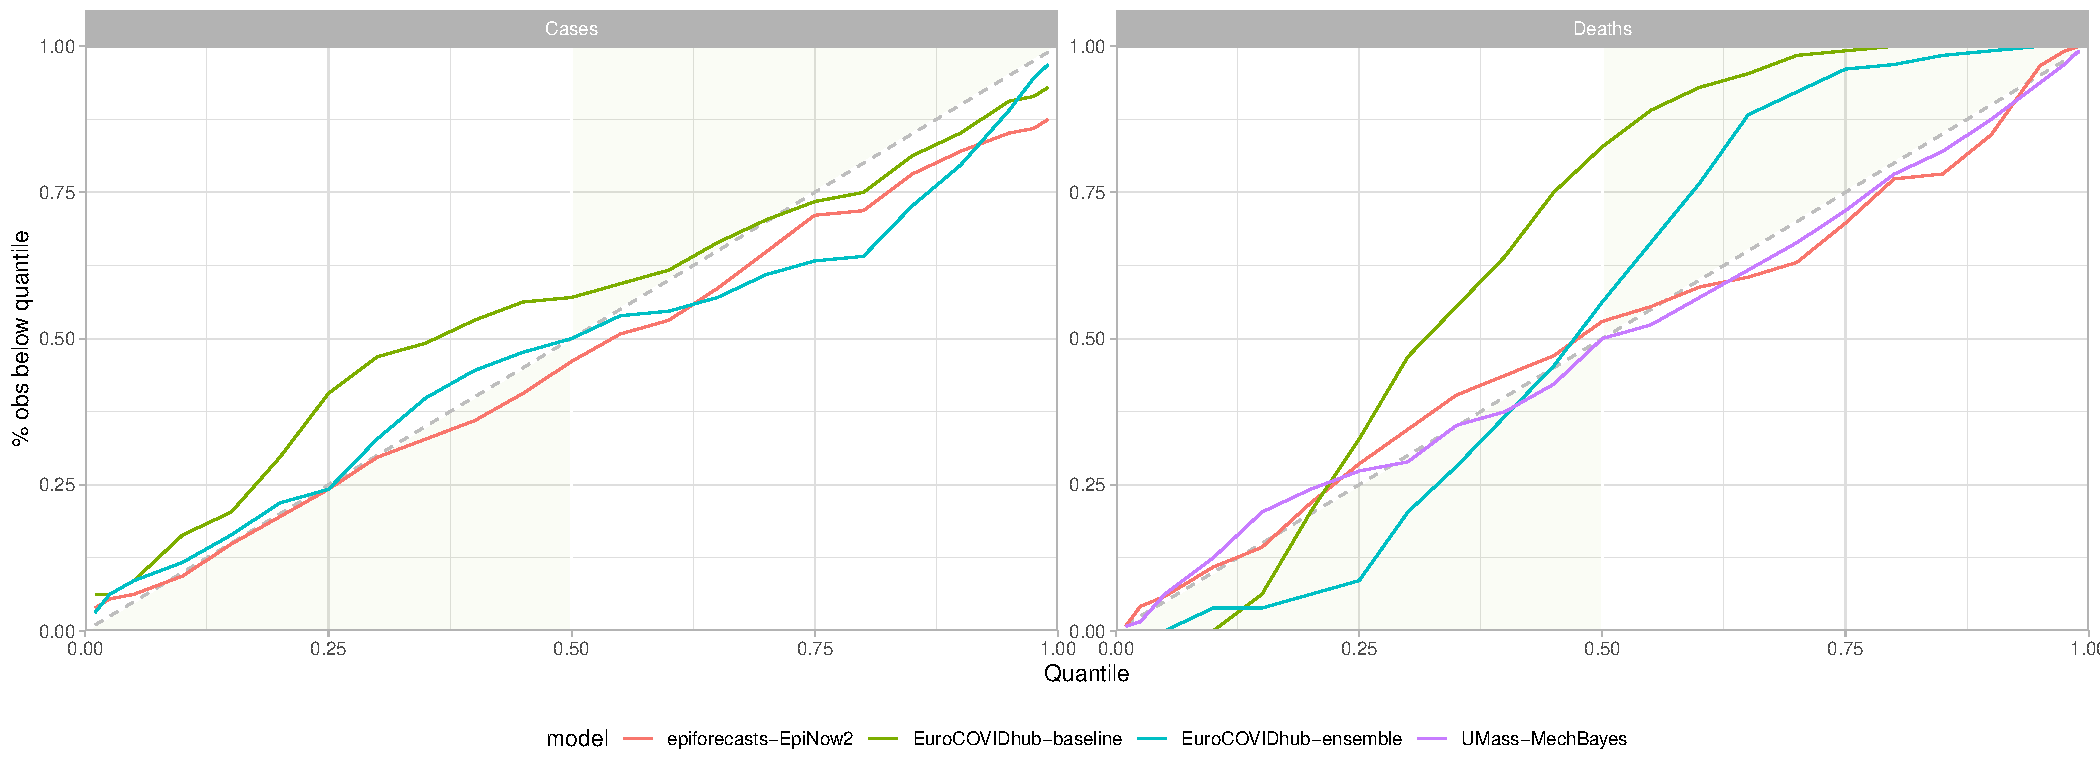
\includegraphics[width=\maxwidth]{plots/plot-quantile-coverage-1} 
\end{knitrout}


\caption{\label{fig:coverage} quantile and interval coverage}
\end{figure}


DO I WANT TO INCLUDE PIT PLOTS AS WELL? I GUESS? NEED TO LOOK AT THE IMPLEMENTATION FOR QUANTILE FORECASTS

% \begin{figure}[h]
% \centering
% <<
% pit-plots, echo=TRUE, fig=TRUE, height=5.2, width=12>>=
% # out <- eval_forecasts(example_quantile, 
% #                       summarise_by = c("model"), 
% #                       pit_plots = TRUE)
% 
% @
% \caption{\label{fig:calibration-pit} pit plots}
% \end{figure}

Look at e.g. bias by location? Figure \ref{fig:bias-heatmap}

\begin{figure}[h]
\centering
\begin{knitrout}
\definecolor{shadecolor}{rgb}{0.969, 0.969, 0.969}\color{fgcolor}\begin{kframe}
\begin{alltt}
\hlstd{> }\hlstd{scores} \hlkwb{<-} \hlkwd{eval_forecasts}\hlstd{(example_quantile,} \hlkwc{summarise_by} \hlstd{=} \hlkwd{c}\hlstd{(}\hlstr{"model"}\hlstd{,}
\hlstd{+ }    \hlstr{"target_type"}\hlstd{,} \hlstr{"location_name"}\hlstd{),} \hlkwc{compute_relative_skill} \hlstd{=} \hlnum{FALSE}\hlstd{)}
\hlstd{> }\hlstd{scoringutils}\hlopt{::}\hlkwd{score_heatmap}\hlstd{(scores,} \hlkwc{metric} \hlstd{=} \hlstr{"interval_score"}\hlstd{,}
\hlstd{+ }    \hlkwc{x} \hlstd{=} \hlstr{"location_name"}\hlstd{,} \hlkwc{facet_formula} \hlstd{=} \hlopt{~}\hlstd{target_type,} \hlkwc{scale} \hlstd{=} \hlstr{"free_x"}\hlstd{)}
\end{alltt}
\end{kframe}
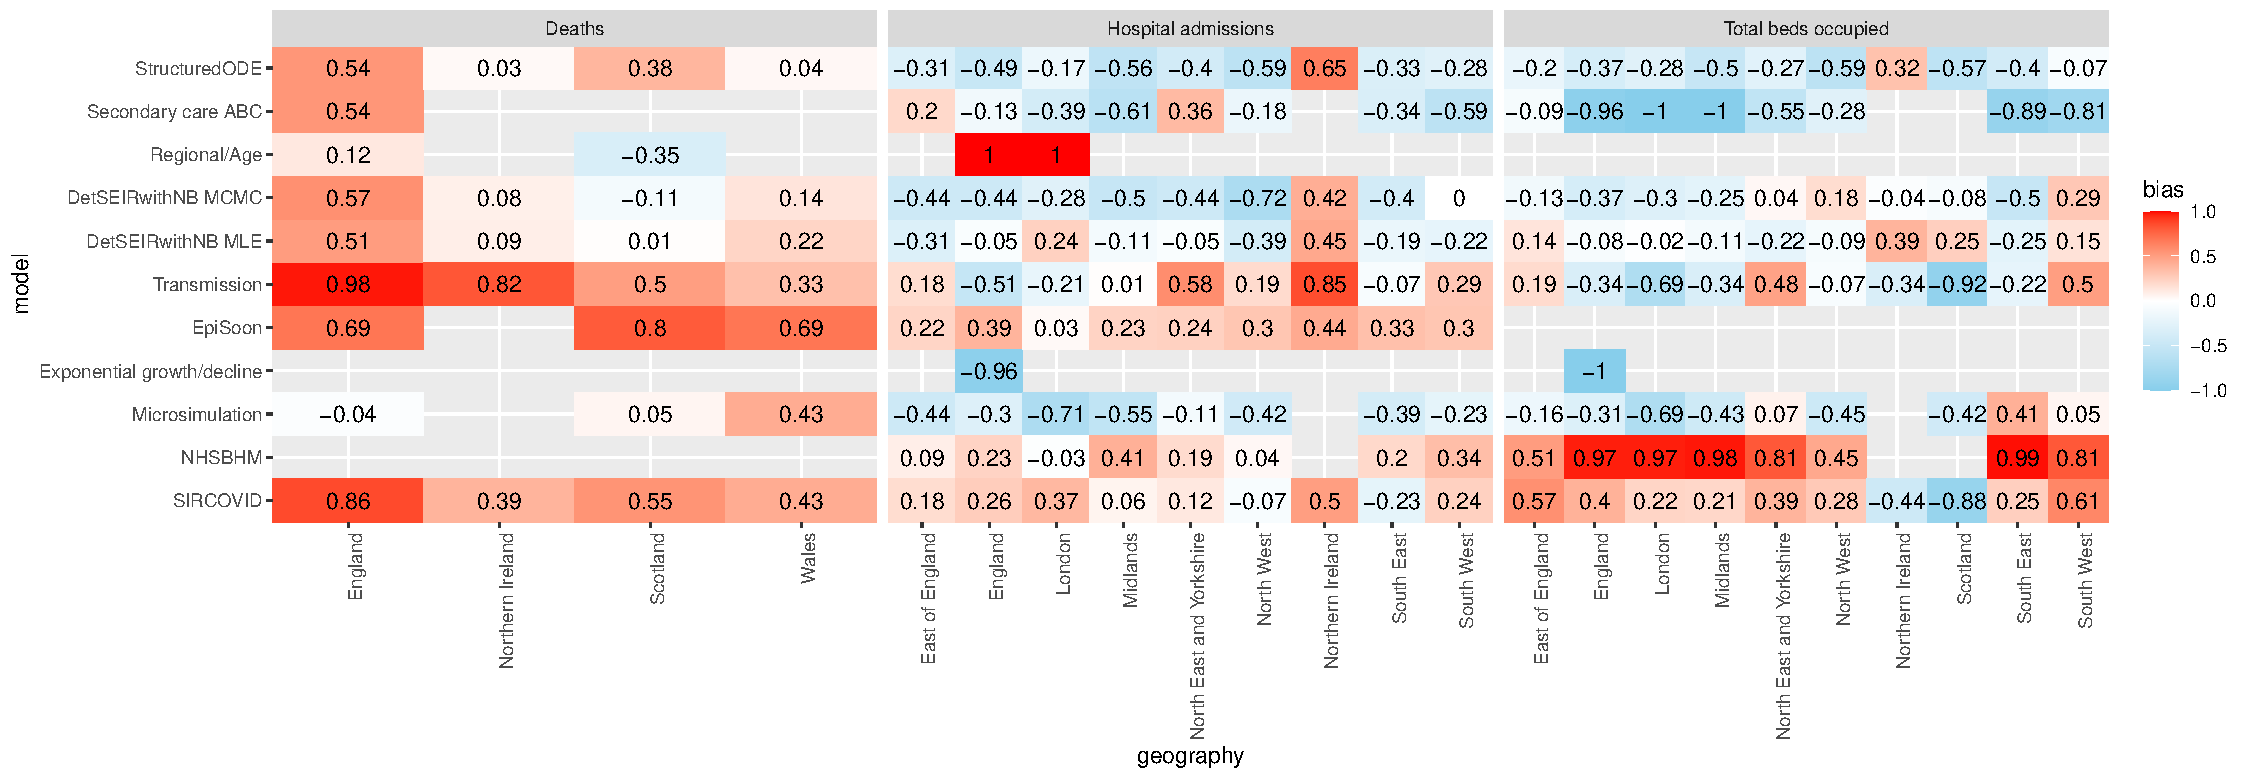
\includegraphics[width=\maxwidth]{plots/plot-calibration-1} 
\end{knitrout}
\caption{\label{fig:bias-heatmap} bias by location}
\end{figure}

WHAT IS NEEDED HERE IS A BIT OF THINKING WITH REGARDS TO WHAT VISUALISATION I WANT TO SHOW AND IN HOW MUCH DETAIL I WANT TO ANALYSE THE MODELS. 


% \begin{CodeInput}
% .
% \end{CodeInput}



%% -- Summary/conclusions/discussion -------------------------------------------

\section{Summary and discussion} \label{sec:summary}

COMING SOON. 


% The results in this paper were obtained using
% \proglang{R}~paste(R.Version()[6:7], collapse = ".") with the
% \pkg{MASS}~packageVersion("MASS") package. \proglang{R} itself
% and all packages used are available from the Comprehensive
% \proglang{R} Archive Network (CRAN) at
% \url{https://CRAN.R-project.org/}.


\section*{Acknowledgments}


% All acknowledgments (note the AE spelling) should be collected in this
% unnumbered section before the references. It may contain the usual information
% about funding and feedback from colleagues/reviewers/etc. Furthermore,
% information such as relative contributions of the authors may be added here
% (if any).


%% -- Bibliography -------------------------------------------------------------
%% - References need to be provided in a .bib BibTeX database.
%% - All references should be made with \cite, \citet, \citep, \citealp etc.
%%   (and never hard-coded). See the FAQ for details.
%% - JSS-specific markup (\proglang, \pkg, \code) should be used in the .bib.
%% - Titles in the .bib should be in title case.
%% - DOIs should be included where available.

\bibliography{scoringutils-paper, references}

%% -- Appendix (if any) --------------------------------------------------------
%% - After the bibliography with page break.
%% - With proper section titles and _not_ just "Appendix".

\newpage

\begin{appendix}

\section{Appendix section} \label{app:technical}

\begin{table}[h!]
\centering

\caption{\label{tab:score-table} Explanation of all the scores}
\end{table}


\end{appendix}

%% -----------------------------------------------------------------------------


\end{document}


%Missing forecasts can have a large impact on the forecast evaluation, if forecasts are not missing at random, but instead missingness correlates with performance.



%BIAS
% For continuous forecasts, assessing whether a predictive distribution has a tendency to over- or underpredict can be very easily achieved by simply evaluating the predictive distribution at the true observed value. This metric is a generalisation of the integer-valued one @funkAssessingPerformanceRealtime2019 have proposed. It is also closely related to the probability integral transform (PIT) discussed later in this chapter. To improve the interpretability of the score we can transform it to a value between -1 (under-prediction) and 1 (over-prediction). Consequently, we measure bias as
% $$B_t (P_t, x_t) = 1 - 2 \cdot (P_t (x_t)),$$
% where $P_t$ is the cumulative distribution function of the predictive distribution for the true value $x_t$. When using predictive samples, $P_t (x_t)$ is simply the fraction of predictive samples for $x_t$ that are smaller than the true observed $x_t$.
% 
% For integer valued forecasts, we use the metric proposed by @funkAssessingPerformanceRealtime2019: 
% $$B_t (P_t, x_t) = 1 - (P_t (x_t) + P_t (x_t + 1)).$$
% Bias can again assume values between -1 (under-prediction) and 1 (over-prediction) and is 0 ideally. 
% 
% For quantile forecasts, we propose the following metric to assess bias: 
% \begin{align*}
%   B_t =& (1 - 2 \cdot \max \{i | q_{t,i} \in Q_t \land q_{t,i} \leq x_t \}) \mathbbm{1}( x_t \leq q_{t, 0.5}) \\
%   &+ (1 - 2 \cdot \min \{i | q_{t,i} \in Q_t \land q_{t,i} \geq x_t\}) \mathbbm{1}( x_t \geq q_{t, 0.5}),
% \end{align*}
% where $Q_t$ is the set of quantiles that form the predictive distribution at time $t$. They represent our belief about what the true value $x_t$ will be. For consistency, we define $Q_t$ such that it always includes the element $q_{t, 0} = - \infty$ and $q_{t,1} = \infty$. $\mathbbm{1}()$ is the indicator function that is $1$ if the condition is satisfied and $0$ otherwise. In clearer terms, $B_t$ is defined as the maximum percentile rank for which the corresponding quantile is still below the true value, if the true value is smaller than the median of the predictive distribution. If the true value is above the median of the predictive distribution, then $B_t$ is the minimum percentile rank for which the corresponding quantile is still larger than the true value. If the true value is exactly the median, both terms cancel out and $B_t$ is zero. For a large enough number of quantiles, the percentile rank will equal the proportion of predictive samples below the observed true value, and this metric coincides with the one for continuous forecasts. 
